%-------------------------------------------------------------------------------
%% outhesis_template.tex
%% version 1.0
%% Chris McRaven <mcraven@physics.ou.edu>
%%
%% 'outhesis.cls' is a class file for a master or phd thesis that
%% conforms to the requirements of the graduate college at the
%% University of Oklahoma. This file is a hacked version of 'book.cls,'
%% that includes all of the formatting requirements set forth in
%% the document 'DissertationInstPacket.pdf' available at
%% http://gradweb.ou.edu/Current/Forms/doctoral/DissertationPagination.pdf
%%
%% This class file relies on a few packages to work.  You must have the
%% following packages installed:
%%  amsfonts, amsmath, amssymb, tikz, lineno, microtype, hyperref
%%
%% Most of these packages are included in distributions of latex.  If you
%% get a lot of errors when compiling, check that these packages are
%% installed.
%%
%% By default, the class file will conform to the requirements, but three
%% options are provided for assistance in proofing the document.
%%
%% linenumbers -- turns on linenumbers in the left margin
%% summarypage -- places a page at the beginning of the document listing 
%%                the number of tables, figures, and bibliography items.
%% hyperlinks -- hyperlinks the citations and references for easier
%%                navigation in the document in a reader which supports
%%                hyperlinks.
%%
%-------------------------------------------------------------------------------

\newcommand*{\ATLASLATEXPATH}{atlas_latex/}

%\documentclass[linenumbers,summarypage,hyperlinks]{outhesis}
%\documentclass[linenumbers,hyperlinks]{outhesis}
\documentclass[hyperlinks]{outhesis}
%\documentclass{outhesis}



%-------------------------------------------------------------------------------
% Extra packages:
%-------------------------------------------------------------------------------
% See doc/atlas-physics.pdf for a list of the defined symbols.
% Default options are:
%   true:  journal, misc, particle, unit, xref
%   false: BSM, hion, math, process, other, texmf
% See the package for details on the options.

%\usepackage{\ATLASLATEXPATH atlasbiblatex} % Style file with biblatex options for ATLAS documents.
\usepackage{\ATLASLATEXPATH atlasphysics} % Useful macros
\usepackage[margin=1.0in]{geometry} % see geometry.pdf on how to lay out the page. There's lots.
%\usepackage{geometry} % see geometry.pdf on how to lay out the page. There's lots.
\usepackage{graphicx}
%\usepackage{subfigure} % obsolete. Use subcaption instead.
\usepackage{subcaption} %These packages gives the author the ability to have subfigures within figures, or subtables within table floats.
\usepackage[labelsep=colon,labelfont=bf,font=singlespacing,width=\textwidth,compatibility=false]{caption}
\usepackage{hyperref} % for url
\usepackage{slashed} % Dirac slash notation
\usepackage{amsmath}
\usepackage{authblk}
\usepackage{multirow}
\usepackage{booktabs} % enable the use of \toprule, \midrule, and \bottomrule
\usepackage{color} % for setting font color
\usepackage{bm} % bold and itatic in math mode


\geometry{a4paper} % or letter or a5paper or ... etc
% \geometry{landscape} % rotated page geometry

%\usepackage[english]{babel}
%\usepackage[utf8x]{inputenc}
%\usepackage{listings}
%\usepackage{textpos}  % for putting logo
%\usepackage{tikz}     % transparent background image
%\usepackage{eurosym}  % euro sign
%\usepackage{appendixnumberbeamer} % count presentation slides only
%\usepackage{pbox} % new line in cell of table
%\usepackage{tabularx} % can change the table width

%\newcommand{\HRule}{\rule{\linewidth}{0.3mm}}

%%%%%
%%%%%
%\usepackage[explicit]{titlesec}
%\usepackage{fix-cm}
%\usepackage{lipsum}
%% numbered
%\titleformat{\chapter}
%  {\normalfont\LARGE\bfseries\filleft}
%  {}
%  {0em}
%  {%
%    \parbox[b]{\dimexpr\linewidth-2.5cm\relax}{#1}\hfill%
%    \parbox[b]{2cm}{\hfill{\fontsize{80}{96}\selectfont\thechapter}}%
%  }
%% unnumbered
%\titleformat{name=\chapter,numberless}
%  {\normalfont\LARGE\bfseries\filleft}
%  {}
%  {0em}
%  {\parbox[b]{\dimexpr\linewidth-2.5cm\relax}{#1}}
%% spacing
%\titlespacing*{\chapter}
%  {0pt}{50pt}{40pt}
%%%%%
%%%%%  


%\usepackage[toc]{appendix}
%\usepackage{xspace}
%\usepackage{multirow,bigdelim}
%\usepackage[compat=1.1.0]{tikz-feynman}

% For a bibliography style, you must have the appropriate .bst file
% \bibliographystyle{apj}
%\bibliographystyle{prsty}
%\bibliographystyle{atlasBibStyleWithTitle}

%\usepackage{thesis-def}


%-------------------------------------------------------------------------------
% Content
%-------------------------------------------------------------------------------
 
%%% BEGIN DOCUMENT
\begin{document}

%% Place Dissertation information here
\author{Yu-Ting Shen}
\university{University of Oklahoma}
\college{Graduate College}
\department{Homer L. Dodge Department of Physics and Astronomy}
\title{This is the thesis title}
\address{Norman, Oklahoma}
\yr{2017}
\dgname{Doctor of Philosophy}
%% List your committee members here
\committee{{Dr. Patrick Skubic, Chair}, Dr. Michael Strauss, {Dr. Ron Kantowski}, Dr. Deborah Watson, {Dr. S. Lakshmivarahan}}

%% Put your dedication here. This is completely optional. Delete it if you don't need it.
\begin{dedication}
%To my past, present, and future family.
    \begin{quotation}
        \raggedright{\emph{`Blood, sweat \& respect. First two you give, last one you earn.''}} \\
        \raggedleft{- Dwayne Johnson} 
    \end{quotation}
\end{dedication}

%% Put your acknowledgements here. This is completely optional. Delete it if you don't need it.
\begin{acknowledgements}
    I would like to thank everyone who has helped me.
%
Especially, thanks to my advisor Patrick Skubic, SS/3L+jets analysis convenor Ximo Poveda Torres, and postdoc Judita Mamu\v{z}i\'{c}.
%
Patrick gave me enough freedom and space to work on projects related to the analysis I was interesting in.
He guided me and gave me a lot of useful feedback in the weekly meeting.
He also helped me handle everything related to the university when I based at CERN for the past three years.
%
Ximo is a very good mentor and friend while I was at CERN.
He always taught me physics, helped me to solve the problems I encountered, and helped me to acclimate myself to my new life at CERN.
Without Ximo's substantial help, I couldn't finish my dissertation smoothly and successfully.
%
Judita kindly agreed to help me work on the NUHM2 interpretation in the Higgsino LSP search after I finished the study on the SS/3L+jets analysis.
Because she had experience regarding the NUHM2 model, she provided me with assistance carrying out the analysis and writing documentation.
%She also helped me to prepare the MC production, HiggsinoFitter scripts, and answered questions from the editorial board.
Without her full support, I could not have finished the NUHM2 study in such a short period.
%
Thanks to all my friends at CERN and OU for the good times we enjoyed together in exploring delicious food, traveling, hiking, bouldering, skiing, and boxing.
Thanks to my ex-girlfriend to warm my heart, to encourage me, and to love me, making me feel happiness in the first half of my Ph.D. life.
Thanks to my brother for taking care of my parents while I am far away from Taiwan.
Finally, many thanks to my parents for everything they bestowed on me.

%I would like to deeply thank all of my teachers and professors over the 20 years of my academic journey, for instilling in me a deep, unquenchable desire to learn. 
%\begin{quotation}
%\raggedright{\emph{``If you don't know, the thing to do is not to get scared, but to learn.''}} \\
%\raggedleft{- Ayn Rand, Atlas Shrugged}
%\end{quotation}

%I would also like to thank all of my family and friends who have helped motivate and encourage me in my pursuit of this degree. 
%\begin{quotation}
%\raggedright{\emph{``It's the job that's never started as takes longest to finish.''}} \\
%\raggedleft{- J.R.R. Tolkien, The Lord of the Rings}
%\end{quotation}

%Lastly, I would like to thank my wife for not only supporting me through the entire process, but actually pushing me to be the best me I could be. Thank you for living this adventure with me!
%\begin{quotation}
%\raggedright{\emph{``I am a wife-made man.''}} \\
%\raggedleft{- Danny Kaye} 
%\end{quotation}
%\begin{quotation}
%\raggedright{\emph{``I knew when I met you an adventure was going to happen.''}} \\
%\raggedleft{- A.A. Milne, Winnie the Pooh} 
%\end{quotation}


\end{acknowledgements}

%% Put your abstract here.
%\begin{abstract}
%   The ATLAS and CMS collaborations announced the discovery of the Higgs boson in July 2012, completing the particle content of the Standard Model.
Although the Standard Model is a great triumph, it is not considered to be the complete theory of particle physics.
%While the physicists try to search for new physics beyond the Standard Model (SM), several new theories have been developed.
Several new theories have been proposed which seek to move beyond the Standard Model.
Among the newly-developed theories, Supersymmetry (SUSY) is one of the most promising ones.
SUSY predicts the existence of supersymmetric partner particles and it is one of the best-motivated extensions of the space-time symmetry of particle interactions.
There are supersymmetric partner particles associated with each SM particles in which the spin differs by 1/2.
This dissertation focuses on a search for electroweak production of supersymmetric particles with compressed mass spectra in the final states with exactly two low-momentum leptons and missing transverse momentum.
The proton-proton collision data is recorded by the ATLAS detector at the Large Hadron Collider in 2015 and 2016, corresponding to 36.1~{\ifb} of integrated luminosity at $\sqrt{s} = 13$~{\TeV}.
Events with same-flavor and opposite electric charge lepton pairs are selected.
The data are found to be consistent with the Standard Model prediction.
Results are interpreted using the non-universal Higgs mass model with two extra parameters (NUHM2) with small mass differences between the masses of produced supersymmetric particles.
Upper limits of the cross-section at 95\% confidence level are set for the NUHM2 model as a function of the universal gaugino mass $m_{1/2}$.

%\end{abstract}

\frontmatter

\maketitle

\mainmatter

\hypersetup{linkcolor=blue}

%% You can put any part of the text in separate file with 
%% the \input{} command. This keeps the master document simpler.

\chapter{Introduction}
\label{chapter:introduction}
\graphicspath{{figures/introduction/}}
The Standard Model of particle physics (SM) describes various phenomena of particle physics.
The discovery of the Higgs boson ($H$) by the ATLAS and CMS collaboration at CERN completes the missing part of the SM prediction~\cite{Aad:2012tfa, Chatrchyan:2012xdj}.
However, there are several open challenges that cannot be explained by the SM, such as hierarchy problem~\cite{Weinberg:1975gm, Gildener:1976ai, Susskind:1978ms} and the dark matter candidate.
In order to answer those questions, a new theory extending the SM is necessary.
Supersymmetry (SUSY)~\cite{Wess:1973kz, Wess:1974tw, Golfand:1971iw, Martin:1997ns} is the most promising extensions of the SM.
SUSY, which is a spacetime symmetry, introduces the superpartners of SM particles (sparticles) with spin differing by one-half unit with respect to the SM partners.
The sparticles provide a potential solution to the hierarchy problem.
If $R$-parity is conserved~\cite{Fayet:1976et, Fayet:1977yc, Farrar:1978xj}, the sparticles are produced in pairs and the lightest SUSY particle (LSP) is stable providing a candidate for dark matter.

The charginos $\widetilde{\chi}^{\pm}_{1,2}$ and neutralinos $\widetilde{\chi}^{0}_{1,2,3,4}$ are the mass eigenstates in the order of increasing masses and collectively referred to as electroweakinos.
They are the mixture of the bino $\widetilde{B}$, winos $\widetilde{W}$, and Higgsinos $\widetilde{H}_{u,d}$ which are the superpartners of the $U(1)$, $SU(2)$ gauge bosons, and the Higgs bosons, respectively.
The charginos and neutralinos can decay into leptons and LSPs via $W$, $Z$, $H$ or sleptons $\widetilde{\ell}$.
In many SUSY models, the lightest neutralino $\widetilde{\chi}^{0}_{1}$ is the LSP.
The LSP would not be detected and results in significant missing transverse energy \MET.

The compressed scenarios refer to the small mass differences between heavier SUSY particles and the LSP.
For example, the mass differences between the heavier electroweakino states $\widetilde{\chi}^{0}_{2}$, $\widetilde{\chi}^{\pm}_{1}$ and the wino- or Higgsino-dominated LSP $\widetilde{\chi}^{0}_{1}$ range from a few {\MeV} to tens of {\GeV} depending on the composition of the mixture.
The $\widetilde{B}$, $\widetilde{W}$, and $\widetilde{H}$ composition of the $\widetilde{\chi}^{0}_{1}$ have an influence on the degree of compression.
Figure~\ref{fig:intro_LSP_composition} shows the composition of the lightest neutralino in a MSSM scan of the electroweakino sector~\cite{Aaboud:2016wna}.
Based on naturalness arguments~\cite{Barbieri:1987fn, deCarlos:1993rbr}, the Higgsino mass parameter $\mu$, the bino and wino mass parameters $M_{1}$ and $M_{2}$ satisfy $|\mu| \ll |M_{1}|, |M_{2}|$ leading to the three electroweakinos $\widetilde{\chi}^{0}_{1}$, $\widetilde{\chi}^{\pm}_{1}$, and $\widetilde{\chi}^{0}_{2}$ being dominated by the Higgsino.

\begin{figure}[htbp]
    \begin{center}
        \includegraphics[scale=1.0]{LSP_composition.pdf}
        \caption{The scatter plot in the $m(\widetilde{\chi}^{0}_{1})$ vs $m(\widetilde{\chi}^{\pm}_{1})$ plane~\cite{Aaboud:2016wna}.
        The color encodes the $\widetilde{\chi}^{0}_{1}$ composition.
        The Higgsino-dominated LSPs are colored in yellow and along the $\widetilde{\chi}^{0}_{1}$-$\widetilde{\chi}^{\pm}_{1}$ diagonal.}
        \label{fig:intro_LSP_composition}
    \end{center}
\end{figure}

This dissertation focuses on searching for electroweak production of SUSY particles in compressed scenarios with exactly two low-momentum same-flavor opposite-charged leptons (electron and muon) in final states and missing transverse momentum $\textbf{p}_{\text{T}}^{\text{miss}}$.
This search uses proton-proton collision data at $\sqrt{s} = 13$~{\TeV} recorded by the ATLAS detector at the Large Hadron Collider (LHC)~\cite{Evans:2008zzb} in 2015 and 2016, corresponding to a total integrated luminosity of 36.1~\ifb.
Figure~\ref{fig:intro_feynman_diagrams} shows the Feynman diagrams representing the electroweakino productions with two leptons final state in association with an initial state radiated jet.
Same-flavor opposite-charged leptons come from the $\widetilde{\chi}^{0}_{2}$ decays in the $\widetilde{\chi}^{0}_{2} \widetilde{\chi}^{\pm}_{1}$ and $\widetilde{\chi}^{0}_{2} \widetilde{\chi}^{0}_{1}$ productions, and from the $\widetilde{\chi}^{\pm}_{1}$ decays in the $\widetilde{\chi}^{\pm}_{1} \widetilde{\chi}^{\mp}_{1}$ production.
The two leptons can be reconstructed in the detector and carry small transverse momentum  \pt.
However, the two LSPs are invisible and back-to-back in the rest frame of their parent electroweakinos.
Because they carry large momentum, the missing transverse energy \met is relatively large.
Similar searches have been performed using $\sqrt{s} = 8$~{\TeV} and $\sqrt{s} = 13$~{\TeV} by the ATLAS~\cite{Aad:2014vma, Aad:2014nua, Aad:2015eda, Aaboud:2016wna} and CMS~\cite{Khachatryan:2014qwa, Khachatryan:2015pot, Sirunyan:2017lae} experiments.
Combining with the results from the LEP experiments, the mass limits for sleptons and charginos are $m(\widetilde{e}_{R}) > 73$~{\GeV}, $m(\widetilde{\mu}_{R}) > 94.6$~{\GeV}, and $m(\widetilde{\chi}^{\pm}_{1}) > 103.5$~{\GeV} or 92.4~{\GeV} depending on the $\Delta m(\widetilde{\chi}^{0}_{1}, \widetilde{\chi}^{\pm}_{1})$.

\begin{figure}[htbp]
    \begin{center}
        \begin{subfigure}[b]{0.32\textwidth}
            \begin{center}
                \includegraphics[scale=1.0]{C1N2-llqqN1N1g-WZ.pdf}
                \caption{The $\widetilde{\chi}^{0}_{2} \widetilde{\chi}^{\pm}_{1}$ production.}
            \end{center}
        \end{subfigure}%
        \begin{subfigure}[b]{0.32\textwidth}
            \begin{center}
                \includegraphics[scale=1.0]{C1C1-llvvN1N1g-WW.pdf}
                \caption{The $\widetilde{\chi}^{\pm}_{1} \widetilde{\chi}^{\mp}_{1}$ production.}
            \end{center}
        \end{subfigure}
        \begin{subfigure}[b]{0.32\textwidth}
            \begin{center}
                \includegraphics[scale=1.0]{N2N1-jllN1N1-Z.pdf}
                \caption{The $\widetilde{\chi}^{0}_{2} \widetilde{\chi}^{0}_{1}$ production.}
            \end{center}
        \end{subfigure}
    \end{center}
    \caption{The Feynman diagrams representing the two leptons final state of (a) $\widetilde{\chi}^{0}_{2} \widetilde{\chi}^{\pm}_{1}$, (b) $\widetilde{\chi}^{\pm}_{1} \widetilde{\chi}^{\mp}_{1}$, (c) $\widetilde{\chi}^{0}_{2} \widetilde{\chi}^{0}_{1}$ productions.}
    \label{fig:intro_feynman_diagrams}
\end{figure}

This dissertation has the following structure.
An introduction is given in Chapter~\ref{chapter:introduction} followed by theoretical foundations in Chapter~\ref{chapter:standard_model} and \ref{chapter:Supersymmetry}.
The experiment facilities are described in Chapter~\ref{chapter:altas_experiment}.
The data and Monte Carlo samples used are detailed in Chapter~\ref{chapter:data}.
Chapter~\ref{chapter:event_reconstruction_and_selection} presents the event reconstruction and the signal region selection.
The background estimation and the systematic uncertainties are discussed in Chapter~\ref{chapter:bkg_estimation}.
The results and interpretation are reported in Chapter~\ref{chapter:results}.
Finally, the conclusions are summarized in Chapter~\ref{chapter:conclusion}.



\chapter{The Standard Model}
\label{chapter:standard_model}
\graphicspath{{figures/standard_model/}}
This chapter outlines the theoretical and mathematical concepts of the high energy particle physics.
The Standard Model of particle physics (SM)~\cite{BF02726525,Glashow,PhysRevLett.19.1264,Herrero:1998eq,CBO9780511791406} is developed since the early 1970s and it has successfully explained almost all experimental results.
The SM is a well-tested and the most successful physics theory to describe the nature of the elementary particles and their interactions.
An overview of the SM is given in Section~\ref{sec:sm}.
After that, an emphasis on the electroweak interactions of the SM is discussed in Section~\ref{sec:ewk}.

%%%
%%%
%%%

\section{The Standard Model of Particle Physics}
\label{sec:sm}
The Standard Model of particle physics is known as the most accurate theory for describing the elementary particles and the interactions between them.
By combining the quantum mechanics and special relativity, the SM is a relativistic \textit{quantum field theory} (QFT) based on a $SU(3)_{C} \otimes SU(2)_{L} \otimes U(1)_{Y}$ symmetry gauge group, where $C$ denotes color, $L$ represents left chirality, and $Y$ stands for weak hypercharge, respectively.
The $SU(3)_{C}$ group is the basis for \textit{Quantum Chromodynamics} (QCD) which describs the strong interaction and the $SU(2)_{L} \otimes U(1)_{Y}$ group is the fundation of the electroweak interaction which unifies the electromatnetic and weak interactions.
Therefore, the SM Lagrangian is invariant under the local gauge transformation.
According to \textit{Noeher's Theorem}~\cite{00411457108231446}, the invariance of an action of a physical system undergoes a symmetry transformation corresponding to a conservation law and vice versa. 
The gauge invariance of the SM Lagrangian corresponds to the conserved quantum numbers, or the charges, of each interaction.
The conserved charges are the three color charge (red, blue, green) for the strong interaction, the third component of the weak isospin $I_{3}^{W}$ for the weak interaction, and the electric charge $Q$ for the electromagnetic interaction.

%%%
%%%
%%%

\subsection{Particle Content}
\label{subsec:sm_particle_content}
According to the SM, all matter around us is made of elementary particles called \textit{quarks} and \textit{leptons}.
The quarks and leptons are called fermions which have half integral spin $s=\frac{1}{2}$, hence the fermions follow the Pauli exclusion principle which says no two fermions have the same quantum state at the same time.
Each fermion has an anti-fermion with the equal mass but carries opposite electric charge, weak isospin and color charge.
There are six quarks and six leptons, they are group into three paris, or "\textit{generations}", ordered by their mass.
The lightest and most stable particles constitute the first generation and they are constituents of ordinary matter.
The heavier and less stable particles form the second and third generations and the heavier particles quickly decay to the next most stable particles.
The three generations of quarks are up ($u$) and down ($d$), charm ($c$) and strange ($s$), and top ($t$) and bottom ($b$) quarks.
The up-type quarks ($u, c, t$) carry $+\frac{2}{3}|e|$ charge and with isospin $+\frac{1}{2}$ while the down-type quarks ($d, s, b$) carry $-\frac{1}{3}|e|$ charge with isospin $-\frac{1}{2}$.
The quarks carry an additional color charge of either red, green, or blue, and hence they only interact via the strong force.
Because the strong force holds quarks together, only non-integer charges of the quark combinations are experimentally allowed.
The quark combinations are called \textit{hadrons} which can be categorised into \textit{mesons} and \textit{baryons}.
The meson is composed by a quark and anti-quark pair ($q\bar{q}$) whereas the baryon is made up by three quarks ($qqq$ or $\bar{q}\bar{q}\bar{q}$).
Only colorless bound states of hadrons are allowed so the quark and anti-quark pair in a meson should contain color and anti-color and the three quarks in a baryon must carry different colors.
The leptons are colorless and are therefore participating in the weak and electromagnetic force only. 
They do not participate in the strong interaction.
The electron-type leptons ($e, \mu, \tau$) carry an elementary charge $|e|$ and their corresponding neutrinos ($\nu_{e}, \nu_{\mu}, \nu_{\tau}$) are neutral.
The neutrinos have very little mass and interact via weak force only.
A summarized table of the properties of quarks and leptons is given in Table~\ref{tab:sm_fermions}.

\begin{table}[htp]
%\begin{center}
\resizebox{\textwidth}{!}{% <------ Don't forget this %
\begin{tabular}{cccccccc}
\hline
\hline
Generation & Fermion & & particle & electric charge $Q$ & weak isospin $I_{3}$ & color charge $C$ & mass [{\GeV}]\\
\hline
\multirow{4}{*}{I} & \multirow{2}{*}{Quark}  & $u$       & up quark          & $+\frac{2}{3}|e|$ & $+\frac{1}{2}$ & r,g,b & 0.0023\\
                   &                         & $d$       & down quark        & $-\frac{1}{3}|e|$ & $-\frac{1}{2}$ & r,g,b & 0.0048\\
                   & \multirow{2}{*}{Lepton} & $e$       & electron          & $-1|e|$           & $-\frac{1}{2}$ & -     & 0.00051\\
                   &                         & $\nu_{e}$ & electron neutrino & 0                 & $+\frac{1}{2}$ & -     & $< 2 \times 10^{-9}$\\
\hline
\multirow{4}{*}{II} & \multirow{2}{*}{Quark}  & $c$         & charm quark   & $+\frac{2}{3}|e|$ & $+\frac{1}{2}$ & r,g,b & 1.275\\
                    &                         & $s$         & strange quark & $-\frac{1}{3}|e|$ & $-\frac{1}{2}$ & r,g,b & 0.095\\
                    & \multirow{2}{*}{Lepton} & $\mu$       & muon          & $-1|e|$           & $-\frac{1}{2}$ & -     & 0.106\\
                    &                         & $\nu_{\mu}$ & muon neutrino & 0                 & $+\frac{1}{2}$ & -     & $< 1.9 \times 10^{-7}$\\
\hline
\multirow{4}{*}{III} & \multirow{2}{*}{Quark}  & $t$          & top quark    & $+\frac{2}{3}|e|$ & $+\frac{1}{2}$ & r,g,b & 173.2\\
                     &                         & $b$          & bottom quark & $-\frac{1}{3}|e|$ & $-\frac{1}{2}$ & r,g,b & 4.18\\
                     & \multirow{2}{*}{Lepton} & $\tau$       & tau          & $-1|e|$           & $-\frac{1}{2}$ & -     & 1.777\\
                     &                         & $\nu_{\tau}$ & tau neutrino & 0                 & $+\frac{1}{2}$ & -     & $< 1.82 \times 10^{-5}$\\

\hline
\hline
\end{tabular}
}
%\end{center}
\caption{The SM fermions with charges and masses~\cite{PDG}.}
\label{tab:sm_fermions}
\end{table}%

%\begin{figure}[htbp]
%\begin{center}
%\includegraphics[scale=0.3]{800px-Standard_Model_of_Elementary_Particles.png}
%\caption{default.
%https://en.wikipedia.org/wiki/Standard_Model
%}
%\label{fig:sm_particles}
%\end{center}
%\end{figure}

%%%
%%%
%%%

Three of the four fundamental forces, strong, weak, electromatnetic forces are parts of the SM now and the gravitational fources could not yet be included in the SM.
Table~\ref{tab:fundamental_forces} shows the four fundamental forces, the relative strength and range together with the theories and the mediators.

\begin{table}[htp]
\begin{center}
\begin{tabular}{ccccc}
\hline
\hline
Force & Rel. Strength & Range (m)& Theory & Mediator\\
\hline
Strong & $10$ & $10^{-15}$ & Chromodynamics & Gluon\\
Weak & $10^{-13}$ & $10^{-18}$ & Flavourdynamics & $W^{\pm}$ and $Z^{0}$ bosons\\
Electromagnetic & $10^{-2}$ & $\infty$ & Electrodynamics & Photon\\
\hline
Gravitational & $10^{-42}$ & $\infty$ & General relativity & Graviton\\
\hline
\hline
\end{tabular}
\end{center}
\caption{The four fundamental forces with the relative strength, interaction range, describing theory, and the mediator.}
\label{tab:fundamental_forces}
\end{table}%

%%%
%%%
%%%

























% Forces and carrier particles

% There are four fundamental forces at work in the universe: the strong force, the weak force, the electromagnetic force, and the gravitational force. They work over different ranges and have different strengths. Gravity is the weakest but it has an infinite range. The electromagnetic force also has infinite range but it is many times stronger than gravity. The weak and strong forces are effective only over a very short range and dominate only at the level of subatomic particles. Despite its name, the weak force is much stronger than gravity but it is indeed the weakest of the other three. The strong force, as the name suggests, is the strongest of all four fundamental interactions.
% Three of the fundamental forces result from the exchange of force-carrier particles, which belong to a broader group called “bosons”. Particles of matter transfer discrete amounts of energy by exchanging bosons with each other. Each fundamental force has its own corresponding boson – the strong force is carried by the “gluon”, the electromagnetic force is carried by the “photon”, and the “W and Z bosons” are responsible for the weak force. Although not yet found, the “graviton” should be the corresponding force-carrying particle of gravity. The Standard Model includes the electromagnetic, strong and weak forces and all their carrier particles, and explains well how these forces act on all of the matter particles. However, the most familiar force in our everyday lives, gravity, is not part of the Standard Model, as fitting gravity comfortably into this framework has proved to be a difficult challenge. The quantum theory used to describe the micro world, and the general theory of relativity used to describe the macro world, are difficult to fit into a single framework. No one has managed to make the two mathematically compatible in the context of the Standard Model. But luckily for particle physics, when it comes to the minuscule scale of particles, the effect of gravity is so weak as to be negligible. Only when matter is in bulk, at the scale of the human body or of the planets for example, does the effect of gravity dominate. So the Standard Model still works well despite its reluctant exclusion of one of the fundamental forces.
% So far so good, but...

% ...it is not time for physicists to call it a day just yet. Even though the Standard Model is currently the best description there is of the subatomic world, it does not explain the complete picture. The theory incorporates only three out of the four fundamental forces, omitting gravity. There are also important questions that it does not answer, such as “What is dark matter?”, or “What happened to the antimatter after the big bang?”, “Why are there three generations of quarks and leptons with such a different mass scale?” and more. Last but not least is a particle called the Higgs boson, an essential component of the Standard Model.
% On 4 July 2012, the ATLAS and CMS experiments at CERN's Large Hadron Collider (LHC) announced they had each observed a new particle in the mass region around 126 GeV. This particle is consistent with the Higgs boson but it will take further work to determine whether or not it is the Higgs boson predicted by the Standard Model. The Higgs boson, as proposed within the Standard Model, is the simplest manifestation of the Brout-Englert-Higgs mechanism. Other types of Higgs bosons are predicted by other theories that go beyond the Standard Model.
% On 8 October 2013 the Nobel prize in physics was awarded jointly to François Englert and Peter Higgs "for the theoretical discovery of a mechanism that contributes to our understanding of the origin of mass of subatomic particles, and which recently was confirmed through the discovery of the predicted fundamental particle, by the ATLAS and CMS experiments at CERN's Large Hadron Collider."
% So although the Standard Model accurately describes the phenomena within its domain, it is still incomplete. Perhaps it is only a part of a bigger picture that includes new physics hidden deep in the subatomic world or in the dark recesses of the universe. New information from experiments at the LHC will help us to find more of these missing pieces.



\chapter{Suppersymmetry}
\label{chapter:Suppersymmetry}
\graphicspath{{figures/susy/}}
The Standard Model of particle physics (SM)~\cite{BF02726525,0029-55826190469-2,PhysRevLett.19.1264,Herrero:1998eq,CBO9780511791406} gets a stupendous success in expecting and explaining the physics phenomena of the elementary particles.
However, the Standard Model leaves several open questions unanswered as mentioned in Section~\ref{sec:sm_bsm}.
Many different models of new physics were proposed to explain those unanswered questions.
Among these new models, the \textit{supersymmetry} (SUSY)~\cite{Wess:1974tw,Lykken:1996xt,Drees:1996ca,Martin:1997ns,Bilal:2001nv,Argyres:2001eva,Peskin:2008nw,CBO9780511619250,Shadmi:2017qdk} wins most physicists' favour.
The SUSY proposed by Wess and Zumino~\cite{Wess:1974tw} at early 1970s is a symmetry relating bosonic and fermionic degrees of freedom.
It extends the Standard Model by requiring every SM boson/fermion has a fermonic/bosonic supersymmetric partner and vice versa.
The reason why physicists favour SUSY is described in Section~\ref{sec:susy_why_susy}.  
The introduction of the SUSY is given in Section~\ref{sec:susy_intro} and the formulaism is depicted in Section~\ref{sec:susy_}.
The \textit{Radiative Natural SUSY} (RNS) and the \textit{Non-Universal Higgs Mass model} with two extra parameters (NUHM2) are given in Section~\ref{sec:susy_rns} and ~\ref{sec:susy_nuhm2}, respectively.

%%%
%%%
%%%

\section{Why supersymmetry}
\label{sec:susy_why_susy}
The Standard Model leaves several unanswered questions, for example, the hierarchy problem (Section~\ref{subsec:sm_hierarchy_problem}), what is the candidates of dark matter (Section~\ref{subsec:sm_dm}), and why don't the running coupling constants unify at GUT level (Section~\ref{subsec:sm_grand_unification}).
The SUSY provides good explanations for these questions.

%%%
%%%
%%%

\subsubsection{Hierarchy problem}
\label{subsubsec:susy_hierarchy_problem}
The Standard Model expects the Higgs squared mass divergent at the Plank scale $\sim 10^{19}$~{\GeV}.
However, the $W^{\pm}$ and $Z^{0}$ gauge bosons obtained their finite mass through the Higgs mechanism indicates the Higgs squared mass must be finite.
The Figure~\ref{fig:susy_one_loop_corrections} shows the Feymann diagram for the one loop correction to the Higgs squared mass due to a fermion $f$ and a scalar $S$.

\begin{figure}[htbp]
\begin{center}
\includegraphics[scale=0.5]{Figure-1-One-loop-quantum-corrections-to-the-Higgs-squared-mass-parameter-m-2-H-from.png}
\caption{The Feymann diagram for the one loop correction to the Higgs squared mass due to (a) a fermion $f$ and (b) a scalar $S$.
The figure is taken from~\cite{Martin:1997ns}.}
\label{fig:susy_one_loop_corrections}
\end{center}
\end{figure}

The corrections are
%
\begin{align}
\Delta m_{H}^{2} &= - \frac{|\lambda_{f}^{2}|}{8\pi^{2}} \Lambda_{UV}^{2} + \cdots, \quad \mathrm{fermion}\\
\Delta m_{H}^{2} &= \frac{\lambda_{S}}{16\pi^{2}} \Lambda_{UV}^{2} + \cdots, \quad \mathrm{boson}
\end{align}
%
where the $\Lambda_{UV}$ is an ultraviolet momentum cutoff which is valid up to the Plank scale $10^{19}$~{\GeV}.
The corrections diverge when $\Lambda_{UV}$ becoming very large.
Because the contributions from the fermion and scalar loops have opposite sign, the divergence contributions can be canceled out if there is a scalar loop for each fermonic loop.
The SUSY predicts the existence of the bosonic/fermonic sparticles, therefore, if $\lambda_{S} = 2 |\lambda_{f}^{2}|$ then the SUSY maintain the finiteness of the Higgs squared mass in a natural way.

%%%
%%%
%%%

\subsubsection{Dark matter}
\label{subsubsec:susy_dark_matter}
The dark matter (DM) makes up about 27\% of the universe and it might originate from neutral relic from the early universe.
The cosmology observations of the dark matter indicate that the dark mater should be electrically neutral, cold, massive, and it participates only the weak and gravitational interactions.
Therefore, the dark matter candidate should be a new particle which is \textit{weakly interacting massive particle} (WIMP).
The SUSY requires all the sparticles must be produced in pairs and they decay into stable \textit{lightest supersymmetry particles} (LSP) with odd number.
If there are a lot of sparticles produced in the early Universe, they will have to decayed to LSPs and remain until the present day because the LSP is stable.
The LSP is a weakly interacting massive particle.
It doesn't interact electromagnetically so they cannot be scattered by photon and thus dark.
There are 3 kinds of LSP could be the possible dark matter candidate, the lightest \textit{neutralino}, the lightest \textit{sneutrino} and the \textit{gravitino}.

%%%
%%%
%%%

\subsubsection{Grand Unification}
\label{subsubsec:susy_gut}
The Grand Unified Theory (GUT) tries to unify the strong and electroweak interactions.
There will be only one interaction and one coupling constant at the GUT scale ($\approx 10^{16}$~{\GeV}).
However, the current coupling constants for electromagnetic, weak, and strong interactions don't unified at the GUT scale as shown in the left hand side of Figure~\ref{fig:sm_coulping_constants}.
This problem can be solved by introducing the SUSY which modifies the renormalization group equations and make the running gauge couplings converged at the GUT scale.
The right hand side of Figure~\ref{fig:sm_coulping_constants} shows the running gauge couplings in SUSY.

%%%
%%%
%%%

\section{Introduction of the supersymmetry}
\label{sec:susy_intro}
An brief overview of the SUSY are introduced in this section.
Firstly, the mathematical foundation of the SUSY, superalgebra, is described in Section~\ref{subsec:susy_superalgebra} followed by the superspace and superfields in Section~\ref{subsec:susy_superspace_and_superfields}.

%%%
%%%
%%%

\subsection{Superalgebra}
\label{subsec:susy_superalgebra}
The SUSY is based on the superalgebra which is an extension of space-time Poincar\'{e} algebra.
The Poincar\'{e} group is a product of the Lorentz group and the group of translations in space-time.
A Lorentz group must satisfies the commutation relations
%
\begin{equation}
[J^{+}_{i}, J^{+}_{j}] = i \epsilon_{ijk} J^{+}_{k}, \quad 
[J^{-}_{i}, J^{-}_{j}] = i \epsilon_{ijk} J^{-}_{k}, \quad 
[J^{+}_{i}, J^{-}_{j}] = 0
\label{eq:susy_Lorentz_commutation_relations}
\end{equation}
%
where $i, j, k = 1, 2, 3$.
If the six Lorentz group generators are combined into an antisymmetric second rank tensor generator $M_{\mu\nu}$ where $M_{ij} = \epsilon_{ijk}J_{k}$ and $M_{0i} = -M_{i0} = -K_{i}$\footnote{The $J_{i}$ and $K_{i}$ with $i=1,2,3$ are rotation and boost generators in 3-dimension respectively.} and the generator of the translation groups is $P_{\mu}$, the energy-momentum operator, then the commutation relations of the Poincar\'{e} group are
%
\begin{align}
[P_{\mu}, P_{\nu}] &= 0 ,\\
[M_{\mu \nu}, P_{\lambda}] &= i (g_{\nu \lambda} P_{\mu} - g_{\mu \lambda} P_{\nu}) ,\\
[M_{\mu \nu}, M_{\rho \sigma}] &= -i (g_{\mu \rho} M_{\nu \sigma} - g_{\mu \sigma} M_{\nu \rho} - g_{\nu \rho} M_{\mu \sigma} + g_{\nu \sigma} M_{\mu \rho}) .
\label{eq:susy_Poincare_commutation_relations}
\end{align}
where the metric is 
\begin{equation}
g_{\mu \nu} =
\left(
\begin{array}{cccc}
1 & 0 & 0 & 0\\
0 & -1 & 0 & 0\\
0 & 0 & -1 & 0\\
0 & 0 & 0 & -1   
\end{array}
\right)
\label{eq:susy_metric}
\end{equation}
%
A general spin 1/2 particle state, $\chi$, can be expressed as a \textit{spinor} in the SUSY using two-component spin up $\chi_{+}$ and spin down $\chi_{-}$ column matrices
%
\begin{equation}
\chi = c_{+} \chi_{+} + c_{-} \chi_{-}
= c_{+} \left(\begin{matrix}1\\0\end{matrix}\right) + c_{-} \left(\begin{matrix}0\\1\end{matrix}\right)
= \left(\begin{matrix}c_{+}\\c_{-}\end{matrix}\right)
\label{eq:susy_spinor}
\end{equation}
%
The solution of the Dirac equation\footnote{The Dirac equation is $(i \gamma^{\mu} \partial_{\mu} - m)\psi = 0$.}, $\psi_{D}\footnote{The Dirac spinor, $\psi_{D}$, is a four-component field which can be expressed using a four-component matrix.}$, can be expressed using the left-handed and right-handed \textit{Weyl spinors} $\psi_{L}$ and $\psi_{R}$ 
%
\begin{equation}
\psi_{D} = \left(\begin{matrix}\psi_{1}\\\psi_{2}\\\psi_{3}\\\psi_{4}\end{matrix}\right)
= \left(\begin{matrix} \left(\begin{matrix}\psi_{1}\\\psi_{2}\end{matrix}\right) \\ \left(\begin{matrix}\psi_{3}\\\psi_{4}\end{matrix}\right) \end{matrix}\right)
= \left(\begin{matrix}\psi_{L}\\\psi_{R}\end{matrix}\right)
\label{eq:susy_Dirac_spinor}
\end{equation}
%

%%%
%%%
%%%

\subsection{Superspace and superfields}
\label{subsec:susy_superspace_and_superfields}

%%%
%%%
%%%

\subsection{$R$-parity}
\label{subsec:susy_r_parity}
The baryon number $B$ and lepton number $L$ are conserved in the Standard Model but violated in the SUSY.
Therefore, a new symmetry called $R$-parity is introduced to eliminate the $B$ and $L$ violating term.
The $R$-parity is defined as
%
\begin{equation}
R \equiv (-1)^{3(B-L)+2s}
\label{eq:susy_r_parity}
\end{equation}
%
where $s$ is the spin of the particle.
All of the SM particles have even $R$-parity ($R$ = +1), while all of the sparticles have odd $R$-parity ($R$ =  1). 
If the $R$-parity is conserved, SUSY predicts that sparticles are produced in pairs in collider experiments.

%%%
%%%
%%%

\subsection{Soft suppersymmetry breaking}
%%%
%%%
%%%

\subsection{The Minimal Supersymmetry Standard Model}
\label{subsec:susy_mssm}
The Minimal Supersymmetry Standard Model (MSSM) is the minimal extension of the Standard Model.
The MSSM contains only the smallest number of superfields and interactions such that the Standard Model particles can keep their current forms.

%%%
%%%
%%%

\subsubsection{Particle content}
\label{subsubsec:susy_particle_content}
%The anticommuting SUSY generator, $Q$, changes the bosons/fermions into fermions/bosons
%\begin{equation}
%Q |\mathrm{boson}\rangle = |\mathrm{fermion}\rangle, \quad Q|\mathrm{fermion}\rangle = |\mathrm{boson}\rangle
%\label{eq:susy_generator}
%\end{equation}
All the super particles, \textit{\textbf{s}particles}\footnote{The super particles of the SM fermions are prefix a "\textit{\textbf{s}}" and the super particles of the SM bosons are suffix an "\textit{\textbf{ino}}". A tilde is added on the symbol of the SM particle to denote its super partner.}, have exactly the same quantum number as their SM particles except the spins differ by $\frac{1}{2}$.
The super partners of the leptons and quarks are called \textit{\textbf{s}leptons} and \textit{\textbf{s}quarks}.
The sleptons and squarks are scalar particles with spin $s=0$ and the left-handed and right-handed states are treated as different particles such that the SM particles and the SUSY \textbf{s}particles have the same number of degree of freedom.
The super partners of gluons are \textit{glu\textbf{ino}s} and there are eight gluinos with spin $s=\frac{1}{2}$. 
The super partners of the gauge bosons $W^{\pm}, Z^{0}$, and $\gamma$, are \textit{gaug\textbf{ino}s}.
The gauginos have spin $s = \frac{1}{2}$.
The super partners of the Higgs bosons\footnote{The Higgs sector contains two charged states $H^{\pm}$ and three neutral states $h^{0}, H^{0}$, and $A^{0}$. The $h^{0} and H^{0}$ are $CP$ even state and $A^{0}$ is $CP$ odd state.} are \textit{Higgs\textbf{ino}s}.
The Higgsinos and gauginos mixing states are two \textit{charginos} $\tilde{\chi}_{1}^{\pm}, \tilde{\chi}_{2}^{\pm}$ and four \textit{neutralinos} $\tilde{\chi}_{1}^{0}, \tilde{\chi}_{2}^{0}, \tilde{\chi}_{3}^{0}, \tilde{\chi}_{4}^{0}$ with spin $s=\frac{1}{2}$.
Table~\ref{tab:susy_particle_contents} shows the particle contents in the MSSM.

\begin{table}[htp]
%\begin{center}
\resizebox{\textwidth}{!}{% <------ Don't forget this %
\begin{tabular}{ccccccc}
\hline
\hline
Supermultiplet & Names & Symbol & spin 0 & spin 1/2 & spin 1 & $SU(3)_{C} \otimes SU(2)_{L} \otimes U(1)_{Y}$\\
\hline
\multirow{3}{*}{Chiral} & \multirow{3}{3cm}{squarks, quarks ($\times 3$ families)} &Q & ($\widetilde{u}_{L}$, \quad $\widetilde{d}_{L})$ & $(u_{L}, \quad d_{L})$ & - & $\mathbf{3} \otimes \mathbf{2}\otimes \frac{1}{6}$\\
& & $\overline{u}$ & $\widetilde{u}^{*}_{R}$ & $u^{\dag}_{R}$ & - & $\overline{\mathbf{3}} \otimes \mathbf{1} \otimes -\frac{2}{3}$\\
& & $\overline{d}$ & $\widetilde{d}^{*}_{R}$ & $d^{\dag}_{R}$ & - & $\overline{\mathbf{3}} \otimes \mathbf{1} \otimes \frac{1}{3}$\\
\hline
\multirow{2}{*}{Chiral} & \multirow{2}{3cm}{sleptons, leptons ($\times 3$ families)} & L & $(\widetilde{\nu}, \quad \widetilde{e}_{L})$ & $(\nu, \quad e_{L})$ & - & $\mathbf{1} \otimes \mathbf{2} \otimes -\frac{1}{2}$\\
& & $\overline{e}$ & $\widetilde{e}^{*}_{R}$ & $e^{\dag}_{R}$ & - & $\mathbf{1} \otimes \mathbf{1} \otimes 1$\\
\hline
\multirow{2}{*}{Chiral}  & \multirow{2}{*}{Higgs, higgsinos} & $H_{u}$ & $(H^{+}_{u}, \quad H^{0}_{u})$ & $(\widetilde{H}^{+}_{u}, \quad \widetilde{H}^{0}_{u})$ & - & $\mathbf{1} \otimes \mathbf{2} \otimes +\frac{1}{2}$\\
& & $H_{d}$ & $(H^{0}_{d}, \quad H^{-}_{d})$ & $(\widetilde{H}^{0}_{d}, \quad \widetilde{H}^{-}_{d})$ & - & $\mathbf{1} \otimes \mathbf{2} \otimes -\frac{1}{2}$\\
\hline
\hline
\multirow{3}{*}{Gauge} & gluino, gluon & - & - & $\widetilde{g}$ & $g$ & $\mathbf{8} \otimes \mathbf{1} \otimes 0$\\
& winos, $W$ bosons & - & - & $\widetilde{W}^{\pm}$, $\widetilde{W}^{0}$ & $W^{\pm}$, $W^{0}$ & $\mathbf{1} \otimes \mathbf{3} \otimes 0$\\
& bino, $B$ boson & - & - & $\widetilde{B}^{0}$ & $B^{0}$ & $\mathbf{1} \otimes \mathbf{1} \otimes 0$\\
\hline
\hline
\end{tabular}
%\end{center}
}
\caption{Chiral supermultiplets and gauge supermultiplets in the MSSM.
In the chiral supermultiplets, the spin 0 fields are complex scalars and the spin 1/2 fields are left-handed two-component Weyl spinors.}
\label{tab:susy_particle_contents}
\end{table}%


 

%%%
%%%
%%%

\section{}
\label{sec:susy_}

%%%
%%%
%%%

\section{The radiative natural SUSY}
\label{sec:susy_rns}

%%%
%%%
%%%

\section{The non-universal Higgs model with two extra parameters}
\label{sec:susy_nuhm2}


\chapter{The ATLAS Experiment at LHC}
\label{chapter:altas_experiment}
\graphicspath{{figures/atlas_experiment/}}
The European Organization for Nuclear Research (CERN\footnote{The name CERN is derived from the acronym for the French Conseil Europ\'{e}en pour la Recherch Nucl\'{e}aire}) was founded in 1954 and is based in the suburb of Geneva on the Franco\textendash Swiss border.
The main function of CERN is to provide particle accelerators and detectors for high-energy physics research.
The physicists and engineers at CERN are probing the fundamental structure of the universe using the world's largest and most complex scientific facility \textemdash \ the Large Hadron Collider (LHC)~\cite{1748-0221-3-08-S08001}.
In the LHC, the particles are boosted to high energies and collide at close to the speed of light.
The results of the collisions are recorded by the various detectors.
There are seven experiments at the LHC.
The biggest of these experiments are ATLAS (A Toroidal LHC ApparatuS)~\cite{1748-0221-3-08-S08003} and CMS (Compact Muon Solenoid)~\cite{1748-0221-3-08-S08004} which use general-purpose detectors to investigate a broad physics programme ranging from the search for the Higgs boson to extra dimensions and particles that could make up dark matter.
The ALICE (A Large Ion Collider Experiment)~\cite{1748-0221-3-08-S08002} experiment is designed to study the physics of quark-gluon plasma form and the LHCb (Large Hadron Collider beauty)~\cite{1748-0221-3-08-S08005} experiment specializes in investigating of CP violation by studying the $b$-quark.
These four detectors sit underground in huge caverns of the LHC ring.
The rest three experiments, TOTEM~\cite{1748-0221-3-08-S08007}, LHCf~\cite{1748-0221-3-08-S08006}, and MoEDAL~\cite{Pinfold:1181486}, are smaller.
The TOTEM (TOTal Elastic and diffractive cross section Measurement)~\cite{1748-0221-3-08-S08007} experiment aims at the measurement of total cross section, elastic scattering, and diffractive dissociation.
The LHCf (Large Hadron Collider forward)~\cite{1748-0221-3-08-S08006} experiment is intended to measure the neutral particle produced by the collider using the forward particles.
The prime motivation of the MoEDAL (Monopole and Exotics Detector at the LHC)~\cite{Pinfold:1181486} experiment is to search directly for the magnetic monopole.

\section{The Large Hadron Collide}
The LHC~\cite{1748-0221-3-08-S08001} is the world's largest and most powerful accelerator which accelerates and collides protons in a 26.7 km circumference crossing the Franco\textendash Swiss border 100 m underground.
The LHC is designed for collisions at a centre-of-mass energy $\sqrt{s}=14$ TeV and an instantaneous luminosity of $\mathcal{L} =10^{34} \ \textrm{cm}^{-2}\textrm{s}^{-1}$.
The first beam was circulated through the collider on the morning of 10 September 2008~\cite{CERN-COURIER-Sep192008}.
However, a magnet quench incident occurred on 19 September 2008 and caused extensive damage to over 50 superconducting magnets, their mountings, and the vacuum pipe.
Most of 2009 was spent on repairs the damage caused by the magnet quench incident and the operations resumed on 20 November of that year.
The first phase of data-taking (Run 1) started at the end of 2009 and the beam energy was increased to a centre-of-mass $\sqrt{s}=7$ TeV in 2011 and $\sqrt{s} = 8$ TeV in 2012.
The total integrated luminosity of 5.46 fb$^{-1}$ was collected in 2011 and of 22.8 fb$^{-1}$ was collected in 2012.
Since 13 February 2013 the LHC was in the Long Shutdown 1 (LS1) phase for maintenance and upgrades.
On 5 April 2015, the LHC restarted and was operating at a centre-of-mass energy $\sqrt{s}=13$ TeV throughout the Run 2 phase (2015 to 2017).



\section{The ATLAS experiment}

\subsection{The Inner Detector}

\subsection{The Calorimeter}

\subsection{The Muon Spectrometer}

\subsection{The Trigger system}

\subsection{}


\chapter{Data set and simulated events}
\label{chapter:data}
\graphicspath{figures/data}
This chapter describes the collision data and simulated event samples used in searching for electroweak production of SUSY states in the compressed scenarios.
The collision data are presented in Sect.~\ref{sec:data_collision_data} and the Monte Carlo (MC) simulated event samples are detailed in Sect.~\ref{sec:data_MC_samples}.
The samples used for searching the strongly-produced SUSY particles in final states with two same-sign or three lepton and jets (SS/3L+jets) can be found in the App.~\ref{sec:app_samples_strong}.


\section{Collision data}
\label{sec:data_collision_data}
The $pp$ collision data used in this analysis were collected by the ATLAS detector at $\sqrt{s} = 13$~{\TeV} during 2015 and 2016 at LHC.
The data corresponds to an integrated luminosity of 36.1 \ifb (3.2 \ifb in 2015 and 32.9 \ifb in 2016) with a combined uncertainty of 2.1\% after applying beam, detector, and data-quality requirements.
The combined uncertainty is derived following the methodology similar to those described in Ref.~\cite{Aaboud:2016hhf}.
The average number of $pp$ interactions per bunch crossing (pile-up) is 13.5 in the 2015 data set and is 25 in the 2016 data set.
The data samples are required to satisfy the following good runs list (GRLs) as recommended by the ATLAS collaboration
%
\begin{itemize}
    \item {\scriptsize \texttt{data15\_13TeV.periodAllYear\_DetStatus-v79-repro20-02\_DQDefects-00-02-02\_PHYS\_StandardGRL\_All\_Good\_25ns.xml}}
    \item {\scriptsize \texttt{data16\_13TeV.periodAllYear\_DetStatus-v88-pro20-21\_DQDefects-00-02-04\_PHYS\_StandardGRL\_All\_Good\_25ns.xml}}
\end{itemize}
%
Events are selected using different inclusive \met triggers depending on the run period as listed in Table.~\ref{tab:data_triggers}.
Two new triggers, \texttt{HLT\_mu4\_j125\_xe90\_mht} and \texttt{HLT\_2mu4\_j85\_xe50\_mht}, are developed for compressed scenarios starting from run number 308084.
However, these new triggers only contribute a small gain compared to the inclusive \met triggers.
This analysis uses inclusive \met triggers only.

\begin{table}[htp]
    \begin{center}
        \begin{tabular}{cc}
            \hline
            \hline
            Run period & \met trigger\\
            \hline
            2015 & \texttt{HLT\_xe70\_mht}\\
            A-D3 & \texttt{HLT\_xe90\_mht\_L1XE50}\\
            D4-F1 & \texttt{HLT\_xe100\_mht\_L1XE50}\\
            F1- & \texttt{HLT\_xe110\_mht\_L1XE50}\\
            \hline
            \hline
        \end{tabular}
    \end{center}
    \caption{The inclusive \met trigger used in this analysis.}
    \label{tab:data_triggers}
\end{table}%

%%%
%%%
%%%

\section{Monte Carlo simulated event samples}
\label{sec:data_MC_samples}
MC samples are used to model the SUSY signals and to estimated the SM background.
All SM background MC samples were processed through a detailed ATLAS detector simulation based on {\GEANT}4~\cite{Agostinelli:2002hh} and the SUSY signal samples were simulated by a fast simulation (AF2) that parameterizes the calorimeter response~\cite{ATLAS:2010bfa}.
To simulate the effects of additional $pp$ collisions (pile-up) in the same and nearby bunch crossings, inelastic interactions were generated using the soft QCD processes of {\PYTHIA} 8.186~\cite{Sjostrand:2007gs} with A2 tune~\cite{ATLAS:2012uec} and the MSTW2008LO PDF set~\cite{Martin:2009iq}.
These MC events were overlaid onto each simulated hard-scatter event and reweighted to match the pile-up conditions observed in the data.

%%%
%%%
%%%

\subsection{The SM background samples}
\label{subsec:data_sm_bkg_samples}
The {\SHERPA} 2.1.1, 2.2.1, and 2.2.2 ~\cite{Gleisberg:2008ta} were used to produce the $Z^{(*)}/\gamma^{*}$ + jets, diboson, and triboson events.
The matrix elements (ME) were calculated for up to two partons at next-to-leading order (NLO) and up to four partons at leading order (LO) depending on the process.
The $Z^{(*)}/\gamma^{*}$ + jets and diboson samples cover the dilepton invarant masses from 0.5~{\GeV} for $Z^{(*)}/\gamma^{*} \to e^{+}e^{-}/\mu^{+}\mu^{-}$ and from 3.8~{\GeV} for $Z^{(*)}/\gamma^{*} \to \tau^{+}\tau^{-}$.
The {\POWHEG}-Box v1 and v2 interfaced to {\PYTHIA} 6.428 were used to simulated \ttbar and single-top production at NLO in the ME.
The Higgs boson production were generated using {\POWHEG}-Box v2 interfaced to {\PYTHIA} 8.186.
A Higgs boson in association with a $W$ or $Z$ boson production was simulated using MG5\_{\scriptsize A}MC@NLO 2.2.2 with {\PYTHIA} 8.186 and the ATLAS A14 tune.
The processes containing \ttbar and at least one electroweak bosons were produced using MG5\_{\scriptsize A}MC@NLO 2.2.1, 2.2.2, 2.3.2, 2.3.3 with {\PYTHIA} 6.4.28 or 8.186.
These processes were generated at NLO in the ME except for $t + Z$ and $t +$ \ttbar which were produced at LO.
Table~\ref{tab:data_mc_samples} summarizes the event generator configurations of the ME, parton shower, PDF set, and the cross-section normalization.
Except those produced by {\SHERPA} event generator, the \textsc{EVTGEN}\xspace v1.2.0~\cite{Lange:2001uf} was used to model the decay of bottom and charm hadrons in all MC samples.

\begin{table}[ht]
    %\begin{center}
    \resizebox{\textwidth}{!}{% <------ Don't forget this %
        \begin{tabular}{lllll}
            \hline
            \hline
            Process                     & Matrix element                                      & Parton shower   & PDF set         & Cross-section\\
            \hline
            $Z^{(*)}/\gamma^{*}$ + jets & \multicolumn{2}{c}{{\SHERPA} 2.2.1}                                   & NNPDF 3.0 NNLO  & NNLO\\
            Diboson                     & \multicolumn{2}{c}{{\SHERPA} 2.1.1 / 2.2.1 / 2.2.2}                   & NNPDF 3.0 NNLO  & Generator NLO\\
            Triboson                    & \multicolumn{2}{c}{{\SHERPA} 2.2.1}                                   & NNPDF 3.0 NNLO  & Generator LO, NLO\\
            \hline
            \ttbar                      & {\POWHEG}-Box v2                                    & {\PYTHIA} 6.428 & NLO CT10        & NNLO + NNLL\\
            $t$ ($s$-channel)           & {\POWHEG}-Box v1                                    & {\PYTHIA} 6.428 & NLO CT10        & NNLO + NNLL\\
            $t$ ($t$-channel)           & {\POWHEG}-Box v1                                    & {\PYTHIA} 6.428 & NLO CT10f4      & NNLO + NNLL\\
            $t + W$                     & {\POWHEG}-Box v1                                    & {\PYTHIA} 6.428 & NLO CT10        & NNLO + NNLL\\
            \hline
            $h(\to \ell\ell, WW)$       & {\POWHEG}-Box v2                                    & {\PYTHIA} 8.186 & NLO CTEQ6L1     & NLO\\
            $h + W/Z$                   & MG5\_{\scriptsize A}MC@NLO 2.2.2                    & {\PYTHIA} 8.186 & NNPDF 2.3 LO    & NLO\\
            \hline
            \ttbar + $W/Z/\gamma^{*}$   & MG5\_{\scriptsize A}MC@NLO 2.3.3                    & {\PYTHIA} 8.186 & NNPDF 3.0 LO    & NLO\\
            \ttbar + $WW$/\ttbar        & MG5\_{\scriptsize A}MC@NLO 2.2.2                    & {\PYTHIA} 8.186 & NNPDF 2.3 LO    & NLO\\
            $t + Z$                     & MG5\_{\scriptsize A}MC@NLO 2.2.1                    & {\PYTHIA} 6.428 & NNPDF 2.3 LO    & LO\\
            $t + WZ$                    & MG5\_{\scriptsize A}MC@NLO 2.3.2                    & {\PYTHIA} 8.186 & NNPDF 2.3 LO    & NLO\\
            $t$ + \ttbar                & MG5\_{\scriptsize A}MC@NLO 2.2.2                    & {\PYTHIA} 8.186 & NNPDF 2.3 LO    & LO\\
            \hline
            \hline
        \end{tabular}
    }
    %\end{center}
    \caption{The MC simulated samples of SM background process.}
    \label{tab:data_mc_samples}
\end{table}%

%%%
%%%
%%%

\subsection{The SUSY signal samples}
\label{subsec:data_susy_signal_samples}
The NUHM2 model allows the masses of the Higgs doublets $m_{H_{u}}$ and $m_{H_{d}}$ differ from the universal scalar mass $m_{0}$ at the GUT scale.
The parameters of the NUHM2 model were fixed to $m_{0} = 5$~{\TeV}, $m_{A} = 1$~{\TeV}, $A_{0} = -1.6 m_{0}$, $\tan\beta = 15$, and $\mu = 150$~{\GeV}.
The parameter $m_{1/2}$ is a free parameter and it is varied from 350 to 800~{\GeV}.
These parameters are choosen based on Ref.~\cite{Baer:2013xua}.
These parameter settings lead to RNS with low EWFT which keeps the Higgs boson mass about 125~{\GeV}, the masses of $\tilde{g}$ and $\tilde{q}$ about {\TeV} scale, and the light Higgsino mass about $\mu$.
The mass spectra and decay branching ratios were calculated using \textsc{IsAJET}\xspace v7.84~\cite{Baer:1999sp}.


\chapter{Event reconstruction and selection}
\label{chapter:event_reconstruction_and_selection}
\graphicspath{figures/event_reconstruction}
Candidate events are required to have at least a reconstructed $pp$ interaction vertex with at least two $\pt > 400$~{\MeV} associated tracks.
The vertex with the largest $\sum \pt^{2}$ of the associated tracks is selected as the primary vertex of the event. 
In this chapter, the various object reconstructions and  identifications in the ATLAS experiment are presented.
The electron, muon, and tau objects are presented in Sect.~\ref{subsec:event_electrons},~\ref{subsec:event_muons}, and~\ref{subsec:event_Taus}, respectively.
Followed by the photons in Sect.~\ref{subsec:event_photons}, jets in Sect.~\ref{subsec:event_jets}, and \met in Sect.~\ref{subsec:event_met}.
Finally, the signal region (SR) selection is described in Sect.~\ref{sec:event_signal_region_selection}.

%%%
%%%
%%%

\section{Object selections}
\label{sec:event_object_selections}
This section presents the object definition and selection in the analysis.
The general object selections for ATLAS are described followed by the specific selections used for this analysis.
The definition of objects used in this analysis are based on the recommendations by Combined Performance groups and are summarized in Table~\ref{tab:event_object_definitions}.
The objects are divided into two categories: preselected and signal objects where signal objects are a subset of preselected objects.
Unless otherwise stated, the recommendations implemented in \texttt{SUSYTools-00-08-69}~\cite{SUSYToolsV8} and \texttt{AnalysisBase 2.4.37}~\cite{AnalysisBase} are used for all the objects.

\begin{table}[ht]
    \begin{center}
        {\scriptsize
            \begin{tabular}{lll}
                \hline
                \hline
                Property           & Preselected object                     & Signal object\\
                \hline
                \textbf{Electrons} &                                        &\\
                Kinematic          & $\pt > 4.5$~{\GeV}                     & $\pt > 4.5$~{\GeV}, $|\eta| < 2.47$ (include crack)\\
                Identification     & \texttt{VeryLooseLLH}                  & \texttt{TightLLH}\\
                Isolation          & -                                      & \texttt{GradientLoose}\\
                Impact parameter   & $|z_{0} \sin\theta| < 0.5$~mm          & $|d_{0}/\sigma(d_{0})| < 5$, $|z_{0} \sin\theta| < 0.5$~mm\\
                Reco algorithm     & Veto \texttt{author==16}               & Veto \texttt{author==16}\\
                \hline
                \textbf{Muons}     &                                        &\\
                Kinematic          & $\pt > 4$~{\GeV}                       & $\pt > 4$~{\GeV}, $|\eta| < 2.5$\\
                Identification     & \texttt{Medium}                        & \texttt{Medium}\\
                Isolation          & -                                      & \texttt{FixedCutTightTrackOnly}\\
                Impact parameter   & $|z_{0} \sin\theta| < 0.5$~mm          & $|d_{0}/\sigma(d_{0})| < 3$, $|z_{0} \sin\theta| < 0.5$~mm\\
                \hline
                \textbf{Jets}
                Kinematic          & $\pt > 20$~{\GeV}, $|\eta| < 4.5$      & $\pt > 30$~{\GeV}, $|\eta| < 2.8$\\
                Clustering         & Anti-$k_{t}$ $R = 0.4$ \texttt{EMTopo} & Anti-$k_{t}$ $R = 0.4$ \texttt{EMTopo}\\
                Pileup mitigation  & -                                      & JVT \texttt{Medium} for $\pt < 60$~{\GeV}, $|\eta| < 2.4$\\
                $b$-tagging        & -                                      & $\pt > 20$~{\GeV}, $|\eta| < 2.5$, \texttt{MV2c10} \texttt{FixedCutBeff} 85\%\\
                \hline
                \hline
            \end{tabular}
        }
    \end{center}
    \caption{Summary of objec definitions used in this analysis.}
    \label{tab:event_object_definitions}
\end{table}%

%%%
%%%
%%%

\subsection{Electrons}
\label{subsec:event_electrons}

%%%
%%%
%%%

\subsubsection{General electron reconstruction and identification}
\label{subsubsec:event_electrons_general}
In the ATLAS experiment, electron\footnote{Electrons and positrons are collectively referred to as electrons.} objects are reconstructed and identified using the information from the ID tracks matched to energy clusters in the ECAL.
Electron candidates with $\pt > 4$~{\GeV} and $|\eta| < 2.47$ are selected using the tag-and-probe method for $Z \to ee$ and $J/\psi \to ee$ processes.
Three likelihood based electron identification algorithms, \texttt{Loose}, \texttt{Medium}, and \texttt{Tight} are applied to determine the signal-like reconstructed electron candidates.
These three identifications use the same variables to define the likelihood discriminant but with different selection criteria.
Depending on the electron identification used, the reconstruction efficiency varies from 78 to 90\% and increases with \met.
The electron isolation varies between 90\% and 99\% depending on the isolation selection criteria.
More detail about the electron reconstruction performance can be found in Ref.~\cite{ATLAS:2016iqc} and a detail description about the electron isolation, which is my authorship project, can be found in the App.~\ref{app:electron_isolation}.

%%%
%%%
%%%

\subsubsection{Specific to this analysis}
\label{subsubsec:event_electrons_specific}
The preselected electrons used in this analysis have to satisfy $\pt > 4.5$~{\GeV} and $|\eta| < 2.47$ and pass the likelihood-based \texttt{VeryLooseLLH} identification.
The electron tracks are required to satisfy the longitudinal impact parameter $|z_{0}\sin\theta| < 0.5$~mm.
The electrons coming from the photon conversion are rejected by veto the \texttt{author==16}.
The signal electrons have a tighter selection criteria.
Besides all the requirements for the preselected electrons, the signal electrons are also required to pass \texttt{TightLLH} identification, \texttt{GradientLoose} isolation, and the transverse impact parameter $|d_{0}/\sigma(d_{0})| < 5$ requirements.

%%%
%%%
%%%

\subsection{Muons}
\label{subsec:event_muons}

%%%
%%%
%%%

\subsubsection{General muon reconstruction and identification}
\label{subsubsec:event_muons_general}
In the ATLAS experiment, muon objects are reconstructed and identified using the information from ID and muon spectrometer in the $\pt > 4$~{\GeV} and $|\eta| < 2.7$ region.
Muon candidates are identified by applying quality requirements to suppress background which mainly come from pion and kion decays.
Four categories of muon identification, \texttt{Medium}, \texttt{Loose}, \texttt{Tight}, and \texttt{High}-\pt are provided for different physics analyses.
The \texttt{Medium} minimizes the systematic uncertainties and is provided as the default selection for muons in ATLAS.
The \texttt{Loose} maximize the reconstruction efficiency and is used for multilepton final state analyses.
The \texttt{Tight} maximize the purity of muons and the \texttt{High}-\pt maximize the momentum resolution for $\pt > 100$~{\GeV}.
The muon reconstruction efficiency is about 99\% in $5 < \pt < 100$~{\GeV} and $|\eta| < 2.5$ phase space.
The muon isolation efficiency varies between 93\% and 100\% depending on the isolation selection criteria.
More detail about the muon reconstruction performance can be found in Ref.~\cite{Aad:2016jkr}.

%%%
%%%
%%%

\subsubsection{Specific to this analysis}
\label{subsubsec:event_muons_specific}
%Similar to the preselected electrons, the preselected muons are reconstructed by combining the tracks information from ID and the muon spectrometer.
The preselected muons used in this analysis have to satisfy $\pt > 4$~{\GeV} and $|\eta| < 2.5$, pass the \texttt{Medium} identification, and require $|z_{0}\sin\theta| < 0.5$~mm on the longitudinal impact parameter.
A tighter requirement is applied on the signal muons which in addition pass the \texttt{FixedCutTightTrackOnly} isolation together with $|d_{0}/\sigma(d_{0})| < 3$ on the transverse impace parameter.

%%%
%%%
%%%

\subsection{Taus}
\label{subsec:event_Taus}

%%%
%%%
%%%

\subsubsection{General $\tau$ reconstruction and identification}
\label{subsubsec:event_taus_general}
The mass of $\tau$ lepton is 1.77~{\GeV} and the decay length is 80~$\mu$m which is too short to make $\tau$ reaches the active region of the ATLAS detector.
The $\tau$ can decay either leptonically ($\tau \to \ell \nu_{\ell}$, $\ell = e, \mu$) or hadronically ($\tau \to$ hadrons + $\nu_{\tau}$).
The hadronic tau decays are about 65\% of all possible decay modes and the decay products contain one charged pions (22\%) or three charged pions (72\%) of all cases.
Tau candidates are seeded by jets using the method described in Ref.~\cite{ATLAS:2017mpa} and they are required to have $\pt > 10$~{\GeV} and $|\eta| < 2.5$ but veto the candidates in the crack region $1.37 < |\eta| < 1.52$.
A boosted decision tree (BDT) based algorithm is used to identify the $\tau$ candidate and to reject backgrounds from quark- and gluon-initiated jets.
Three identifications, \texttt{Loose}, \texttt{Medium}, and \texttt{Tight} are provided with the efficiency 60\%, 55\%, and 45\% for 1-track and 50\%, 40\%, and 30\% for 3-tracks, respectively.
More detail about the $\tau$ lepton reconstruction and identification performance can be found in Ref.~\cite{ATLAS:2017mpa}.

%%%
%%%
%%%

\subsubsection{Specific to this analysis}
\label{subsubsec:event_taus_specific}
The di-tau invariant mass $m_{\tau\tau}$ is used in this analysis and addressed in Sect.~\ref{subsec:event_discriminating_variables}.

%%%
%%%
%%%

\subsection{Photons}
\label{subsec:event_photons}

%%%
%%%
%%%

\subsubsection{General photons reconstruction and identification}
\label{subsubsec:event_photons_general}
In the ATLAS experiment, photons are reconstructed using the tracking information in ID and the energy deposits in the CAL.
To distinguish prompt photons\footnote{Prompt photons are photons not originating from hadron decays} from background photons, the photon identification is based on a set of rectangular cuts on several discriminating variables computed from the energy deposited in the ECAL and from the shower leakage to the HCAL.
The photon identification is separately applied to the converted and unconverted photons with $25 \le E_{\mathrm{T}} \le 1500$~{\GeV} and 4 $|\eta|$ intervals.
Two identifications, \texttt{Loose} and \texttt{Tight}, are provided.
The \texttt{Loose} provides high efficiency with low jet rejection and the \texttt{Tight}, which is recommanded for the analyses by the Combined Performance groups, provides high fake photon rejection and good efficiency.
The \texttt{Tight} identification efficiency starts from 84\% at low $E_{\mathrm{T}}$ and reaches around 98\% in $1.37 < |\eta| < 1.81$ region for the unconverted photons.
Similar to the unconverted photons, the efficiency for the converted photons increases with energy and reaches up to 98\%.
More detail about the photon reconstruction and identification can be found in Ref.~\cite{ATLAS:2011kuc}.

%%%
%%%
%%%

\subsubsection{Specific to this analysis}
\label{subsubsec:event_photons_specific}
Photons are required to pass \texttt{Tight} identification and have $\pt > 25$~{\GeV}.

%%%
%%%
%%%

\subsection{Jets}
\label{subsec:event_jets}

%%%
%%%
%%%

\subsubsection{General jets reconstruction}
\label{subsubsec:event_jets_general}
In the ATLAS experiment, jets are reconstructed using the anti-$k_{t}$ algorithm with radius parameter $R = 0.4$.
The reconstruction algorithm uses calorimeter topological clusters in $|\eta| < 4.5$ as input.
Four jet cleaning selections, \texttt{Looser}, \texttt{Loose}, \texttt{Medium}, and \texttt{Tight}, are provided to reject the background.
The \texttt{Looser} has the highest efficiency, $\sim$99.8\%, and the \texttt{Tight} has the highest background rejection with efficiency 85\% at $\pt = 25$~{\GeV} and 98\% at $\pt > 50$~{\GeV}.
More detail about the jets reconstruction using anti-$k_{t}$ algorithm can be found in Ref.~\cite{Cacciari:2008gp}.

%%%
%%%
%%%

\subsubsection{$b$-tagging}
\label{subsubsec:event_bjets}
In the ATLAS experiment, it is very important to identify jets containing $b$ hadrons from light flavor jets\footnote{The light flavor jets mean jets containing $u$, $d$, $s$, $c$, or gluons.}.
Many $b$-tagging algorithms were developed to maintain high $b$-tagging efficiency of real $b$-jets and to retain very low misidentification efficiency of the light flavor jets.
The new developed multivariable algorithm, MV2, improving the $c$-jet rejection $\sim$40\% at 77\% $b$-tagging efficiency and the rejection power at high $b$-jet \pt is also improved.
More detail about the $b$-tagging can be found in Ref.~\cite{ATL-PHYS-PUB-2015-022, ATL-PHYS-PUB-2016-012}.

%%%
%%%
%%%

\subsubsection{Specific to this analysis}
\label{subsubsec:event_jets_specific}
The preselected jets are reconstructed with the anti-$k_{t}$ algorithm with radius parameter $R = 0.4$ and required $\pt > 20$~{\GeV} and $|\eta| < 4.5$.
Jets with $\pt < 60$~{\GeV} and $|\eta| < 2.4$ are required to satisfy \texttt{Medium} jet vertex tagger requirement which can suppress pileup jets.
The MV2c10 $b$-tagging algorithm with an 85\% efficiency is applied on the preselected jets with $|\eta| < 2.5$.
The signal jets are required to satisfy $\pt > 30$~{\GeV} and $|\eta| < 2.8$.

%%%
%%%
%%%

\subsection{Missing transverse energy}
\label{subsec:event_met}
The missing transverse energy \met is defined as the negative vector sum of \pt of all reconstructed objects including leptons, jets, and soft term as show in Eq.~(\ref{eq:event_met}).
The soft term is constructed from all tracks associated to the primary vertex but not associated with any physics object.
There two kinds of soft term, calorimeter based soft term (CST) and track based soft term (TST) are used in \met calculation.
The CST \met is constructed form the energy deposits in the CAL not associated with hard objects and the TST \met is built form ID tracks which not match to any reconstructed object.
More detail about the \met reconstruction performance can be found in Ref.~\cite{ATL-PHYS-PUB-2015-023}.
%
\begin{equation}
    \met = - (\sum \mathbf{p}_{\mathrm{T}}^{\mathrm{hard}} + \mathbf{p}_{\mathrm{T}}^{\mathrm{soft}})
    \label{eq:event_met}
\end{equation}
%

%%%
%%%
%%%

\subsection{Overlap removal}
\label{subsec:event_overlap_removal}
After preselected objects are reconstructed, an overlap removal procedure is applied to resolve ambiguities between the reconstructed jets and leptons.
The distance $\Delta R$ between two objects is used for overlap removal and $\Delta R$ is defined as
%
\begin{equation}
    \Delta R = \sqrt{(\Delta y)^{2} + (\Delta \phi)^{2}}
\end{equation}
%
where $y$ and $\phi$ are rapidity and azimuthal angle, respectively.
The overlap removal procedure has to follow the steps listed below.
In order to avoid the bremsstrahlung from muons followed by a photon conversion into electron pairs, electron candidate is reomved if it shares the same ID track with a muon object.
Jet is removed from the remaining electrons if $\Delta R(\mathrm{jets}, e) < 0.2$ unless it is a $b$-jet.
If there are less than 3 tracks of jets with $\pt > 500$~{\MeV} and the distance between jets and a muon candidate less than 0.4, i.e. $\Delta R(\mathrm{jets}, \mu) < 0.4$, then the jets are removed.
This step can suppress muon bremsstrahlung.
Finally, the electrons and muons are removed if the $e$ or $\mu$ lie in a distance $\Delta R(\mathrm{jets}, e/\mu) < 0.4$ of the surviving jets so that charm and bottom hadron decays are suppressed.

%%%
%%%
%%%

\section{Signal region selection}
\label{sec:event_signal_region_selection}

%%%
%%%
%%%

\subsection{Discriminating variables}
\label{subsec:event_discriminating_variables}
This section provides the explaniations for various variables used to discriminate signals and background.
%
\begin{itemize}
    \item \textbf{Same flavour opposite sign (SFOS) lepton pair}: This analysis requires exactly two preselected and two signal leptons in the final state.
    These two leptons have to carry the same flavor and with opposite electric charge such as $e^{\pm}e^{\mp}$ and $\mu^{\pm}\mu^{\mp}$.

    \item $\mathbf{\pt^{\ell_{1}}}$ and $\mathbf{\pt^{\ell_{2}}}$: The momentum of leading lepton $\pt^{\ell_{1}} > 5$~{\GeV} is required to suppressed fake/nonprompt leptons background and the threshold of the momentum of subleading lepton $\pt^{\ell_{2}} > 4.5$(4)~{\GeV} for electron (muon) is used to retain signal acceptance.

    \item $\mathbf{\Delta R_{\ell\ell}}$: The dilepton distance is defined as Eq.~(\ref{eq:event_dilepton_distance}).
    %This variable provides good discrimination between the Higgsino and slepton because the dileptons from Higgsinos have small angular separation.
    %However, the leptons originate from the slepton don't have strong restrictions on their angular separation.
    The $\Delta R_{\ell\ell}$ variable, which is required to greater than 0.05, suppresses the leptons originating from photon conversions or muons.
    %
    \begin{equation}
        \Delta R_{\ell \ell} = \sqrt{(\eta_{\ell_{1}} - \eta_{\ell_{2}})^{2} + (\phi_{\ell_{1}} - \phi_{\ell_{2}})^{2}}
        \label{eq:event_dilepton_distance}
    \end{equation}
    %

    \item $\mathbf{m_{\ell\ell}}$: The dilepton invariant mass $m_{\ell\ell}$ is bounded by the mass splitting $m(\widetilde{\chi}^{0}_{2}) - m(\widetilde{\chi}^{0}_{1})$ providing the background suppression power.
    The background originates from on-shell $Z$ decay can be suppressed if the upper bound of $m_{\ell\ell}$ is set to 60~{\GeV} and the contributions from $J/\psi$ are vetoed by required a $3 < m_{\ell\ell} < 3.2$~{\GeV} window.

    \item $\mathbf{\met}$: In order to keep the \met trigger efficiency exceeding 95\%, \met is required to be greater than 200~{\GeV}.

    \item $N_{\mathrm{jet}}$: The number of jets is required to greater than or equal to 1 because of the initial state radiation (ISR) jets.

    \item $\mathbf{\pt^{j_{1}}}$: The momentum of the leading jet is required to greater than 100~{\GeV}.

    \item $\mathbf{\Delta \phi(j_{1}, \pt^{\textbf{miss}})}$: The azimuthal separation between $j_{1}$ and $\mathbf{\pt^{\textrm{miss}}}$ is required to greater than 2 to suppress the QCD and $Z$+jets background.

    \item \textbf{min($\mathbf{\Delta \phi(\textbf{any jet}, \pt^{\textbf{miss}})}$)}: By requiring $\Delta \phi(\textrm{any jet}, \pt^{\textbf{miss}}) > 0.4$, the effect of jet-energy mismeasurement on \met can be reduced.

    \item $\mathbf{N}_{\mathbf{b}\textbf{-jet}}$: Requiring $N_{b\textrm{-jet}} = 0$, the \ttbar and single-top backgrounds can be reduced significantly.

    \item $\mathbf{m_{\tau\tau}}$: The di-tau invariant $m_{\tau\tau}(p_{\ell_{1}}, p_{\ell_{2}}, \mathbf{p}_{\mathrm{T}}^{\mathrm{miss}})$ variable is defined as the signed square root of $m^{2}_{\tau\tau}$.
    The $m_{\tau\tau}$ is used to reconstructed the $Z \to \tau \tau$ process where $\tau$ decays leptonically $\tau \to \ell \nu_{\ell} \nu_{\tau}$.
    Figure~\ref{fig:event_mtautau} shows the $Z$ boson leptonic decay process.
    %
    \begin{figure}[htb]
        \begin{center}
            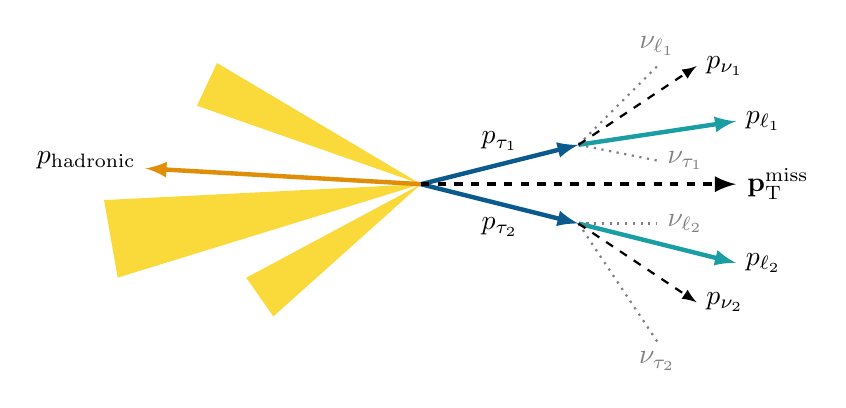
\begin{tikzpicture}

    % jets
    \definecolor{myyellow}{RGB}{249, 209, 9}
    \definecolor{myorange}{RGB}{224, 141, 8}
    \definecolor{myblue}{RGB}{11, 90, 142}
    \definecolor{mygreen}{RGB}{27, 158, 163}
    \definecolor{mylightgreen}{RGB}{186, 225, 226}
    \draw [draw=none, opacity=0.8, fill=myyellow, rotate=10] (0,0) -- (-4,-0.5)-- (-4,0.5) -- (0,0);
    \draw [draw=none, opacity=0.8, fill=myyellow, rotate=-25] (0,0) -- (-3,-0.3)-- (-3,0.3) -- (0,0);
    \draw [draw=none, opacity=0.8, fill=myyellow, rotate=35] (0,0) -- (-2.5,-0.3)-- (-2.5,0.3) -- (0,0);
    
    \draw [-latex, ultra thick, myorange] (0,0)--(-3.5,0.2);
    \node at (-3.5,0.3) [left] {$p_\mathrm{hadronic}$};
    
    % taus
    \draw [-latex, ultra thick, myblue] (0,0)--(2,0.5) ;
    \draw [-latex, ultra thick, myblue] (0,0)--(2,-0.5) ;   
    \node at (1,0.3) [above] {$p_{\tau_1}$};
    \node at (1,-0.3) [below] {$p_{\tau_2}$};
    
    % leptons
    \draw [-latex, ultra thick, mygreen] (2,0.5)--(4,0.8) ;
    \draw [-latex, ultra thick, mygreen] (2,-0.5)--(4,-1) ;      
    \node at (4,0.8) [right] {$p_{\ell_1}$};
    \node at (4,-1) [right] {$p_{\ell_2}$};
    
    % neutrinos
    \draw [dotted, thick, gray] (2,0.5) -- (3,1.5) node [above] {$\nu_{\ell_1}$};
    \draw [dotted, thick, gray] (2,0.5) -- (3,0.3) node [right] {$\nu_{\tau_1}$};
    
    \draw [dotted, thick, gray] (2,-0.5) -- (3,-2) node [below] {$\nu_{\tau_2}$};
    \draw [dotted, thick, gray] (2,-0.5) -- (3,-0.5) node [right] {$\nu_{\ell_2}$};
    
    \draw [-latex, thick, dashed] (2,0.5)--(3.5,1.5) ;
    \draw [-latex, thick, dashed] (2,-0.5)--(3.5,-1.5) ;
    \node at (3.5,1.5) [right] {$p_{\nu_1}$};
    \node at (3.5,-1.5) [right] {$p_{\nu_2}$};
    
    % MET
    \draw [-latex, ultra thick, dashed] (0,0)--(4,0) node [right] {$\mathbf{p}_\mathrm{T}^\mathrm{miss}$};
    
\end{tikzpicture}
            \caption{The illustration of the $Z \to \tau\tau$ + jets decay where $\tau$ decays leptonically $\tau \to \ell \nu_{\ell} \nu_{\tau}$.}
            \label{fig:event_mtautau}
        \end{center}
    \end{figure}
    %
    The $m^{2}_{\tau\tau}$ is defined in Eq.~(\ref{eq:event_mtautua2})
    %
    \begin{equation}
        m^{2}_{\tau\tau} \equiv 2 p_{\ell_{1}} \cdot p_{\ell_{2}} (1 + \xi_{1})(1+ \xi_{2})
        \label{eq:event_mtautua2}
    \end{equation}
    %
    where $p_{\ell_{1}}$ and $p_{\ell_{2}}$ are the momenta of the leptons and the $\xi_{1}$ and $\xi_{1}$ are the scale factor which can be determined by solving $\mathbf{p}_\mathrm{T}^\mathrm{miss} = \xi_{1} \mathbf{p}_\mathrm{T}^{\ell_{1}} + \xi_{2} \mathbf{p}_\mathrm{T}^{\ell_{2}}$.
    From the Eq.~(\ref{eq:event_mtautua2}), the $m^{2}_{\tau\tau}$ can be negative when either $1 + \xi_{1} < 0$ or $1 + \xi_{2} < 0$.
    This situation occurs when only one lepton moves in the same direction as $\mathbf{p}_{hadronic}$ and $|\mathbf{p}_{\ell}|$ is small. 
    This rarely happens for highly boosted $Z \to \tau \tau$ decays but it happens with larger frequency for less boosted heavy particles which decays back-to-back.
    The $m_{\tau\tau}$ is calculated in Eq.~(\ref{eq:event_mtautau}).
    %
    \begin{align}
        m_{\tau\tau} & = \mathrm{sign}(m^{2}_{\tau\tau}) \sqrt{|m^{2}_{\tau\tau}|}\\
                     & = 
                     \begin{cases}
                         \hphantom{-}\sqrt{m_{\tau\tau}^2}    & m_{\tau\tau}^2 \geq 0,\\
                         -\sqrt{\left| m_{\tau\tau}^2\right|} & m_{\tau\tau}^2 < 0.
                     \end{cases}
        \label{eq:event_mtautau}
    \end{align}
    %
    Despite there is a discontinuity at $m_{\tau\tau} = 0$, this variable can be used to discriminate the leptons originating from $Z\to \tau\tau$.

    \item $\mathbf{m_{T}^{\ell_{1}}}$: The transverse mass of \met and the leading lepton is defined in Eq.~(\ref{eq:event_transverse_mass}).
    The \ttbar, $WW/WZ$, and $W$+jets background can be reduced by requiring $m_{\textrm{T}}^{\ell_{1}} < 70$~{\GeV}.
    %
    \begin{equation}
        m_{\textrm{T}}^{\ell_{1}} = \sqrt{2(E_{\textrm{T}}^{\ell_{1}}\met - \mathbf{p}_{\textrm{T}}^{\ell_{1}} \cdot \mathbf{p}_{\textrm{T}}^{\textrm{miss}})}
        \label{eq:event_transverse_mass}
    \end{equation}
    %

    \item $\mathbf{\met/H_{T}^{lep}}$: The scalar sum of the lepton transverse momentum, $H_{\textrm{T}}^{\textrm{lep}}$, is defined  in Eq.~(\ref{eq:event_HT}).
    The $H_{\textrm{T}}^{\textrm{lep}}$ variable has smaller value in the compressed SUSY signal and larger value in the SM background such as $WW$ or $WZ$.
    %
    \begin{equation}
        H_{\textrm{T}}^{\textrm{lep}} = p_{\textrm{T}}^{\ell_{1}} + p_{\textrm{T}}^{\ell_{2}}
        \label{eq:event_HT}
    \end{equation}
    %
    The leptons coming from SM background, for example, \ttbar and diboson are harder but they are softer in the compressed SUSY signal events.
    Therefore, for a given value of \met, the $\met/H_{\textrm{T}}^{\textrm{lep}}$ variable is larger in the compressed signals but is smaller for the background.
    The minimal requirement of this variable is defined in Eq.~(\ref{eq:event_METOverHT}) which is adjusted event by event depending on the mass splitting.
    %
    \begin{equation}
        \met/H_{\textrm{T}}^{\textrm{lep}} > \mathrm{max}[5, 15 - 2 m_{\ell\ell}/(1~{\GeV})]
        \label{eq:event_METOverHT}
    \end{equation}
    %
    Figure~\ref{fig:event_METOverHT} shows the $\met/H_{\textrm{T}}^{\textrm{lep}}$ requirement for the electroweakino SR after applying all the SR common requirements and the $\Delta R_{\ell\ell} < 2$.
    %
    \begin{figure}[htb]
        \begin{center}
            \includegraphics[scale=0.4]{fig_03a.pdf}
            \caption{The distribution of $\met/H_{\textrm{T}}^{\textrm{lep}}$ as function of $m_{\ell\ell}$ for the electroweakino after applying all the SR common requirements and the $\Delta R_{\ell\ell} < 2$.
            The red line indicates the SR selection.
            Events in the region below this line are rejected.
            The signal events are labled in colored circles for different mass splitting.}
            \label{fig:event_METOverHT}
        \end{center}
    \end{figure}
    %
\end{itemize}
%

%%%
%%%
%%%

\subsection{Signal region}
\label{subsec:event_signal_region}
The event selection criteria for the SR are summarized in Table~\ref{tab:event_signal_region} and the $m_{\ell\ell}$ binnings are listed in Table~\ref{tab:event_signal_region_binning}.
There are 14 exclusive regions and 7 inclusive regions are defined.
The exclusive regions are used to set model-dependent limits while the inclusive regions are used to set the model-independent upper limits.
When derive the exclusion limits on the signal model, the SR$ee$-$m_{\ell\ell}$ and SR$\mu\mu$-$m_{\ell\ell}$ regions are combined and fit simultaneously.

\begin{table}[htb]
    \begin{center}
        {\scriptsize
            \begin{tabular}{ll}
                \hline
                \hline
                Variable                                                               & Common requirement\\
                \hline
                Number of leptons                                                      & = 2\\
                Lepton charge and flavor                                               & $e^{+}e^{-}$ or $\mu^{+}\mu^{-}$\\
                Leading lepton $\pt^{\ell_{1}}$                                        & $> 5$~{\GeV} for electron and muon\\
                Subleading lepton  $\pt^{\ell_{2}}$                                    & $> 4.5$ (4)~{\GeV} for electron (muon)\\
                $\Delta R_{\ell \ell}$                                                 & $> 0.05$\\
                $m_{\ell \ell}$                                                        & $\in$ [1, 60]~{\GeV} excluding [3.0, 3.2]~{\GeV}\\
                \met                                                                   & $> 200$~{\GeV}\\
                Number of jets                                                         & $\ge 1$\\
                Leading jet \pt                                                        & $> 100$~{\GeV}\\
                $\Delta \phi(j_{1}, \mathbf{p}^{\mathrm{miss}}_{\mathrm{T}})$          & $> 2.0$\\
                min($\Delta \phi($any jet, $\mathbf{p}^{\mathrm{miss}}_{\mathrm{T}}))$ & $> 0.4$\\
                Number of $b$-tagged jets                                              & = 0\\
                $m_{\tau \tau}$                                                        & $< 0$ or $> 160$~{\GeV}\\
                \hline
                                                                                       & Electroweakino SRs\\
                \hline
                $\Delta R_{\ell \ell}$                                                 & $< 2$\\
                $m_{T}^{\ell_{1}}$                                                     & $< 70$~{\GeV}\\
                $\met/H_{\mathrm{T}}^{\mathrm{lep}}$                                   & $>$ max(5, 15 - 2 $\frac{m_{\ell \ell}}{1~{\GeV}}$)\\
                Binned in                                                              & $m_{\ell \ell}$\\ 
                \hline
                \hline
            \end{tabular}
        }
    \end{center}
    \caption{Summary of event selection criteria.
    Signal leptons and signal jets are used when applying all requirements.
    The SR binning is listed in Table~\ref{tab:event_signal_region_binning}.}
    \label{tab:event_signal_region}
\end{table}%

\begin{table}[htb]
    \begin{center}
        {\scriptsize
            \begin{tabular}{lllllllll}
                \hline
                \hline
                \multicolumn{9}{c}{Electroweakino SRs}\\
                \hline
                Exclusive & SR$ee$-$m_{\ell \ell}$, SR$\mu\mu$-$m_{\ell \ell}$ & [1, 3] & [3.2, 5] & [5, 10] & [10, 20] & [20, 30] & [30, 40] & [40, 60]\\
                Inclusive & SR$\ell \ell$-$m_{\ell \ell}$                      & [1, 3] & [1, 5]   & [1, 10] & [1, 20]  & [1, 30]  & [1, 40]  & [1, 60]\\
                \hline
                \hline
            \end{tabular}
        }
    \end{center}
    \caption{The SR binnings for the electroweakino SRs.
    The SR is defined by a $m_{\ell \ell}$ range in {\GeV}.
    The exclusive bins are used to set the exclusion limits on the model and the inclusive bins are used to set the model-independent limits.}
    \label{tab:event_signal_region_binning}
\end{table}%


\chapter{Background estimation}
\label{chapter:bkg_estimation}
\graphicspath{figures/bkg_estimation}


\section{Irreducible background}
\label{sec:bkg_irreducible_background}

%%%
%%%
%%%

\section{Reducible background}
\label{sec:bkg_reducible_background}

%%%
%%%
%%%

\section{Systematic uncertainties}
\label{sec:bkg_systematic_uncertainties}

%%%
%%%
%%%

\begin{table}[ht]
    \begin{center}
        {\scriptsize
            \begin{tabular}{llll}
                \hline
                \hline
                Region               & Leptons                                                                        & $\met/H_{\mathrm{T}}^{\mathrm{lep}}$                & Additional requirements\\
                \hline
                CR-top               & $e^{\pm}e^{\mp}$, $\mu^{\pm}\mu^{\mp}$, $e^{\pm}\mu^{\mp}$, $\mu^{\pm}e^{\mp}$ & $> 5$                                               & $\ge 1 b$-tagged jet(s)\\
                CR-tau               & $e^{\pm}e^{\mp}$, $\mu^{\pm}\mu^{\mp}$, $e^{\pm}\mu^{\mp}$, $\mu^{\pm}e^{\mp}$ & $\in$ [4, 8]                                        & $m_{\tau \tau} \in$ [60, 120]~{\GeV}\\
                \hline
                VR-VV                & $e^{\pm}e^{\mp}$, $\mu^{\pm}\mu^{\mp}$, $e^{\pm}\mu^{\mp}$, $\mu^{\pm}e^{\mp}$ & $< 3$                                               &\\
                VR-SS                & $e^{\pm}e^{\mp}$, $\mu^{\pm}\mu^{\mp}$, $e^{\pm}\mu^{\mp}$, $\mu^{\pm}e^{\mp}$ & $> 5$                                               &\\
                VRDF-$m_{\ell \ell}$ & $e^{\pm}\mu^{\mp}$, $\mu^{\pm}e^{\mp}$                                         & $>$ max(5, 15 - 2 $\frac{m_{\ell \ell}}{1~{\GeV}}$) & $\Delta R_{\ell \ell} < 2$, $m_{\mathrm{T}}^{\ell_{1}} < 70$~{\GeV}\\
                \hline
                \hline
            \end{tabular}
        }
    \end{center}
    \caption{Definition of control regions and validation regions.}
    \label{tab:bkg_}
\end{table}%

\chapter{Results}
\label{chapter:results}
\graphicspath{figures/results}
This chapter presents the results of the searching for electroweak production of supersymmetric states in NUHM2 compressed scenario.
The kinematic distributions of the NUHM2 are shown in Sect.~\ref{sec:results_kinematic_distributions}.
The $m_{\ell \ell}$ reweighting method is described in Sect.~\ref{sec:results_mll_reweighting}.
The results of the NUHM2 interpretation using the $m_{\ell \ell}$ reweighting method is given in Sect.~\ref{subsec:results_mll_reweighting_interpretation} and the interpretation using the MC production is detailed in Sect.~\ref{sec:results_mc_production_interpretation}.

%%%
%%%
%%%

\section{Kinematic distributions}
\label{sec:results_kinematic_distributions}
The realistic NUHM2 model and the simplified Higgsino model are similar except the $m_{\widetilde{\chi}^{\pm}_{1}}$ is not exactly half way between $m_{\widetilde{\chi}^{0}_{2}}$ and $m_{\widetilde{\chi}^{0}_{1}}$.
The ratio between the $\Delta m(\widetilde{\chi}^{0}_{2}, \widetilde{\chi}^{0}_{1})$ and $\Delta m(\widetilde{\chi}^{\pm}_{1}, \widetilde{\chi}^{0}_{1})$ varies from 1.61 to 1.21 as shown in Table~\ref{tab:data_mass_splitting_ratio}.
The sensitivity of the NUHM2 model used for the two leptons final state Higgsino analysis is examined by comparing the kinematic distributions of the NUHM2 signal samples and the simplied Higgsino model grid mass points.
% Figures~\ref{fig:results_nuhm2_lepton_multiplicity} to \ref{fig:results_nuhm2_met_METOverHTLep12_Rll_dphiMin1} show the kinematic distribution comparisons in TRUTH level using the NUHM2 samples with $m_{1/2} = 600$~{\GeV} and the simplified Higgsino samples with $m_{\widetilde{\chi}^{0}_{2}} = 170$~{\GeV}, $m_{\widetilde{\chi}^{0}_{1}} = 150$~{\GeV}.
Figures~\ref{fig:results_kinematic_distribution_comparisons} shows some of the kinematic distribution comparisons in TRUTH level using the NUHM2 samples with $m_{1/2} = 600$~{\GeV} and the simplified Higgsino samples with $m_{\widetilde{\chi}^{0}_{2}} = 170$~{\GeV}, $m_{\widetilde{\chi}^{0}_{1}} = 150$~{\GeV}.
The distributions for the other kinematic variable comparison can be found in the App.~\ref{app:distributions}.
All events are selected after applying the event cleaning pre-selections and satisfying the $\ge 2$ leptons with $\pt > 3$~{\GeV} and $\met > 50$~{\GeV} requirements.
All kinematic distributions in the truth level are very similar between two models.
The largest difference is in the $m_{\ell \ell}$ distribution due to the mass spliting $\Delta m = m_{\widetilde{\chi}^{0}_{2}} - m_{\widetilde{\chi}^{0}_{1}}$ where $\Delta m \sim 22$~{\GeV} for NUHM2 and 20~{\GeV} for the simplified Higgsino model.
This distinguish feature motivates the NUHM2 interpretation.

\begin{figure}[htbp]
    \begin{center}
        \begin{subfigure}[b]{0.48\textwidth}
            \includegraphics[scale=0.35]{nSignalLeptons.pdf}
            \caption{Signal leptons multiplicities}
        \end{subfigure}
        \begin{subfigure}[b]{0.48\textwidth}
            \includegraphics[scale=0.35]{signalElectrons_pt.pdf}
            \caption{Signal electrons \pt}
        \end{subfigure}
        \begin{subfigure}[b]{0.48\textwidth}
            \includegraphics[scale=0.35]{nJets.pdf}
            \caption{Jets multiplicity}
        \end{subfigure}
        \begin{subfigure}[b]{0.48\textwidth}
            \includegraphics[scale=0.35]{signalJets_pt.pdf}
            \caption{Signal jets \pt.}
        \end{subfigure}
        \begin{subfigure}[b]{0.48\textwidth}
            \includegraphics[scale=0.35]{met.pdf}
            \caption{\met}
        \end{subfigure}
        \begin{subfigure}[b]{0.48\textwidth}
            \includegraphics[scale=0.35]{mll.pdf}
            \caption{$m_{\ell\ell}$}
        \end{subfigure}
    \end{center}
    \caption{The kinematic distribution comparisons in TRUTH level using the NUHM2 samples with $m_{1/2} = 600$~{\GeV} and the simplified Higgsino samples with $m_{\widetilde{\chi}^{0}_{2}} = 170$~{\GeV}, $m_{\widetilde{\chi}^{0}_{1}} = 150$~{\GeV}.
    Four different production channels, $\widetilde{\chi}^{0}_{2}\widetilde{\chi}^{0}_{1}$, $\widetilde{\chi}^{0}_{2}\widetilde{\chi}^{+}_{1}$, $\widetilde{\chi}^{0}_{2}\widetilde{\chi}^{-}_{1}$, and $\widetilde{\chi}^{\pm}_{1}\widetilde{\chi}^{\mp}_{1}$, for the NUHM2 and the simplified Higgsino model are considered.
    The distributions of four productions are combined and normalized to equal area.}
    \label{fig:results_kinematic_distribution_comparisons}
\end{figure}

% \begin{figure}[htbp]
%     \begin{center}
%         \begin{subfigure}[b]{0.48\textwidth}
%             \includegraphics[scale=0.4]{nBaselineLeptons.pdf}
%             \caption{Baseline leptons multiplicities}
%         \end{subfigure}
%         \begin{subfigure}[b]{0.48\textwidth}
%             \includegraphics[scale=0.4]{nSignalLeptons.pdf}
%             \caption{Signal leptons multiplicities}
%         \end{subfigure}
%         \begin{subfigure}[b]{0.48\textwidth}
%             \includegraphics[scale=0.4]{nElectrons.pdf}
%             \caption{Signal electrons multiplicities}
%         \end{subfigure}
%         \begin{subfigure}[b]{0.48\textwidth}
%             \includegraphics[scale=0.4]{nMuons.pdf}
%             \caption{Signal muons multiplicities}
%         \end{subfigure}
%     \end{center}
%     \caption{The lepton multiplicity distributions.
%     The lepton multiplicity of NUHM2 with $m_{1/2} = 600$~{\GeV} are compared to the simplified Higgsino model with $m_{\widetilde{\chi}^{0}_{2}}=170$~{\GeV} and $m_{\widetilde{\chi}^{0}_{1}}=150$~{\GeV}.
%     Four different production channels, $\widetilde{\chi}^{0}_{2}\widetilde{\chi}^{0}_{1}$, $\widetilde{\chi}^{0}_{2}\widetilde{\chi}^{+}_{1}$, $\widetilde{\chi}^{0}_{2}\widetilde{\chi}^{-}_{1}$, and $\widetilde{\chi}^{\pm}_{1}\widetilde{\chi}^{\mp}_{1}$, for the NUHM2 and the simplified Higgsino model are considered.
%     The distributions of four productions are combined and normalized to equal area.}
%     \label{fig:results_nuhm2_lepton_multiplicity}
% \end{figure}

% \begin{figure}[htbp]
%     \begin{center}
%         \begin{subfigure}[b]{0.48\textwidth}
%             \includegraphics[scale=0.4]{nJets.pdf}
%             \caption{Jets multiplicity}
%         \end{subfigure}
%         \begin{subfigure}[b]{0.48\textwidth}
%             \includegraphics[scale=0.4]{nBjets.pdf}
%             \caption{$b$-jets multiplicity}
%         \end{subfigure}
%         \begin{subfigure}[b]{0.48\textwidth}
%             \includegraphics[scale=0.4]{nJet25.pdf}
%             \caption{Signal jets multiplicity with $\pt > 25$~{\GeV}}
%         \end{subfigure}
%         \begin{subfigure}[b]{0.48\textwidth}
%             \includegraphics[scale=0.4]{nJet30.pdf}
%             \caption{Signal jets multiplicity with $\pt > 30$~{\GeV}}
%         \end{subfigure}
%     \end{center}
%     \caption{The jets multiplicity distributions.
%     The jet multiplicity of NUHM2 with $m_{1/2} = 600$~{\GeV} are compared to the simplified Higgsino model with $m_{\widetilde{\chi}^{0}_{2}}=170$~{\GeV} and $m_{\widetilde{\chi}^{0}_{1}}=150$~{\GeV}.
%     The top left plot includes the forward jets and the bottom two plots use the signal jets with $\pt > 25$~{\GeV} and $\pt > 30$~{\GeV}, respectively.
%     Four different production channels, $\widetilde{\chi}^{0}_{2}\widetilde{\chi}^{0}_{1}$, $\widetilde{\chi}^{0}_{2}\widetilde{\chi}^{+}_{1}$, $\widetilde{\chi}^{0}_{2}\widetilde{\chi}^{-}_{1}$, and $\widetilde{\chi}^{\pm}_{1}\widetilde{\chi}^{\mp}_{1}$, for the NUHM2 and the simplified Higgsino model are considered.
%     The distributions of four productions are combined and normalized to equal area.}
%     \label{fig:results_nuhm2_jets_multiplicity}
% \end{figure}

% \begin{figure}[htbp]
%     \begin{center}
%         \begin{subfigure}[b]{0.48\textwidth}
%             \includegraphics[scale=0.35]{signalElectrons_pt.pdf}
%             \caption{Signal electrons \pt}
%         \end{subfigure}
%         \begin{subfigure}[b]{0.48\textwidth}
%             \includegraphics[scale=0.35]{signalMuons_pt.pdf}
%             \caption{Signal muons \pt}
%         \end{subfigure}
%         \begin{subfigure}[b]{0.48\textwidth}
%             \includegraphics[scale=0.35]{signalElectrons_eta.pdf}
%             \caption{Signal electrons $\eta$}
%         \end{subfigure}
%         \begin{subfigure}[b]{0.48\textwidth}
%             \includegraphics[scale=0.35]{signalMuons_eta.pdf}
%             \caption{Signal muons $\eta$}
%         \end{subfigure}
%         \begin{subfigure}[b]{0.48\textwidth}
%             \includegraphics[scale=0.35]{signalElectrons_phi.pdf}
%             \caption{Signal electrons $\phi$}
%         \end{subfigure}
%         \begin{subfigure}[b]{0.48\textwidth}
%             \includegraphics[scale=0.35]{signalMuons_phi.pdf}
%             \caption{Signal muons $\phi$}
%         \end{subfigure}
%     \end{center}
%     \caption{The \pt, $\eta$, and $\phi$ distributions for the NUHM2 with $m_{1/2} = 600$~{\GeV} and the simplified Higgsino model with $m_{\widetilde{\chi}^{0}_{2}}=170$~{\GeV} and $m_{\widetilde{\chi}^{0}_{1}}=150$~{\GeV}.
%     The signal electrons \pt, $\eta$, and $\phi$ distributions are on the left column and the signal muons distributions are on the right.
%     Four different production channels, $\widetilde{\chi}^{0}_{2}\widetilde{\chi}^{0}_{1}$, $\widetilde{\chi}^{0}_{2}\widetilde{\chi}^{+}_{1}$, $\widetilde{\chi}^{0}_{2}\widetilde{\chi}^{-}_{1}$, and $\widetilde{\chi}^{\pm}_{1}\widetilde{\chi}^{\mp}_{1}$, for the NUHM2 and the simplified Higgsino model are considered.
%     The distributions of four productions are combined and normalized to equal area.}
%     \label{fig:results_nuhm2_leptons_pt_eta_phi}
% \end{figure}

% \begin{figure}[htbp]
%     \begin{center}
%         \begin{subfigure}[b]{0.48\textwidth}
%             \includegraphics[scale=0.35]{signalJets_pt.pdf}
%             \caption{The signal jets \pt.}
%         \end{subfigure}
%         \begin{subfigure}[b]{0.48\textwidth}
%             \includegraphics[scale=0.35]{signalBjets_pt.pdf}
%             \caption{The signal $b$-jets \pt.}
%         \end{subfigure}
%         \begin{subfigure}[b]{0.48\textwidth}
%             \includegraphics[scale=0.35]{signalJets_eta.pdf}
%             \caption{The signal jets $\eta$.}
%         \end{subfigure}
%         \begin{subfigure}[b]{0.48\textwidth}
%             \includegraphics[scale=0.35]{signalBjets_eta.pdf}
%             \caption{The signal $b$-jets $\eta$.}
%         \end{subfigure}
%         \begin{subfigure}[b]{0.48\textwidth}
%             \includegraphics[scale=0.35]{signalJets_phi.pdf}
%             \caption{The signal jets $\phi$.}
%         \end{subfigure}
%         \begin{subfigure}[b]{0.48\textwidth}
%             \includegraphics[scale=0.35]{signalBjets_phi.pdf}
%             \caption{The signal $b$-jets $\phi$.}
%         \end{subfigure}
%     \end{center}
%     \caption{The signal jets and the signal $b$-jets \pt, $\eta$, and $\phi$ distributions for the NUHM2 with $m_{1/2} = 600$~{\GeV} and the simplified Higgsino model with $m_{\widetilde{\chi}^{0}_{2}}=170$~{\GeV} and $m_{\widetilde{\chi}^{0}_{1}}=150$~{\GeV}.
%     Four different production channels, $\widetilde{\chi}^{0}_{2}\widetilde{\chi}^{0}_{1}$, $\widetilde{\chi}^{0}_{2}\widetilde{\chi}^{+}_{1}$, $\widetilde{\chi}^{0}_{2}\widetilde{\chi}^{-}_{1}$, and $\widetilde{\chi}^{\pm}_{1}\widetilde{\chi}^{\mp}_{1}$, for the NUHM2 and the simplified Higgsino model are considered.
%     The distributions of four productions are combined and normalized to equal area.}
%     \label{fig:results_nuhm2_jets_bjets_pt_eta_phi}
% \end{figure}

% \begin{figure}[htbp]
%     \begin{center}
%         \begin{subfigure}[b]{0.48\textwidth}
%             \includegraphics[scale=0.4]{mll.pdf}
%             \caption{$m_{\ell\ell}$}
%         \end{subfigure}
%         \begin{subfigure}[b]{0.48\textwidth}
%             \includegraphics[scale=0.4]{MTauTau.pdf}
%             \caption{$m_{\tau\tau}$}
%         \end{subfigure}
%         \begin{subfigure}[b]{0.48\textwidth}
%             \includegraphics[scale=0.4]{mT.pdf}
%             \caption{$m_{T}$}
%         \end{subfigure}
%         \begin{subfigure}[b]{0.48\textwidth}
%             \includegraphics[scale=0.4]{mT2.pdf}
%             \caption{$m_{T2}$}
%         \end{subfigure}
%     \end{center}
%     \caption{The invariant mass $m_{\ell\ell}$ and $m_{\tau\tau}$ distributions and the transverse mass $m_\mathrm{T}$ and $m_\mathrm{T2}$ distributions.
%     The first two leading baseline leptons are used to calculate the $m_{\ell\ell}$ which contains a hump and a tail region.
%     The $\widetilde{\chi}^{0}_{2} \widetilde{\chi}^{0}_{1}$ contributes to the hump only and the tail is contributed by the decay products containing the chargino $\widetilde{\chi}^{\pm}_{1}$.
%     The Eq.~(\ref{eq:event_mtautau}) is used to calculate the di-tau invariant mass $m_{\tau\tau}$.
%     The first or first two leading signal leptons and \met are used to evaluate the transverse mass $m_\mathrm{T}$ and $m_\mathrm{T2}$, respectively.
%     Four different production channels, $\widetilde{\chi}^{0}_{2}\widetilde{\chi}^{0}_{1}$, $\widetilde{\chi}^{0}_{2}\widetilde{\chi}^{+}_{1}$, $\widetilde{\chi}^{0}_{2}\widetilde{\chi}^{-}_{1}$, and $\widetilde{\chi}^{\pm}_{1}\widetilde{\chi}^{\mp}_{1}$, for the NUHM2 and the simplified Higgsino model are considered.
%     The distributions of four productions are combined and normalized to equal area.}
%     \label{fig:results_nuhm2_mll_mtautau_mT_mT2}
% \end{figure}

% \begin{figure}[htbp]
%     \begin{center}
%         \begin{subfigure}[b]{0.48\textwidth}
%             \includegraphics[scale=0.4]{met.pdf}
%             \caption{\met}
%         \end{subfigure}
%         \begin{subfigure}[b]{0.48\textwidth}
%             \includegraphics[scale=0.4]{METOverHTLep12.pdf}
%             \caption{$\met/H_\mathrm{T}^\mathrm{lepton}$}
%         \end{subfigure}
%         \begin{subfigure}[b]{0.48\textwidth}
%             \includegraphics[scale=0.4]{Rll.pdf}
%             \caption{$\Delta R(\ell_{1}, \ell_{2})$}
%         \end{subfigure}
%         \begin{subfigure}[b]{0.48\textwidth}
%             \includegraphics[scale=0.4]{dphiMin1.pdf}
%             \caption{$\Delta \phi(\met, j_{1})$}
%         \end{subfigure}
%     \end{center}
%     \caption{The \met, $\met/H_\mathrm{T}^\mathrm{lepton}$, $\Delta R(\ell_{1}, \ell_{2})$, and $\Delta \phi(\met, j_{1})$ distributions.
%     The $H_\mathrm{T}^\mathrm{lepton}$ is the scalar sum of the first two leading baseline leptons \pt only.
%     The distance $\Delta R(\ell_{1}, \ell_{2})$ is calculated by the first two leading baseline leptons and the $\Delta \phi(\met, j_{1})$ uses \met and first leading signal jet.
%     Four different production channels, $\widetilde{\chi}^{0}_{2}\widetilde{\chi}^{0}_{1}$, $\widetilde{\chi}^{0}_{2}\widetilde{\chi}^{+}_{1}$, $\widetilde{\chi}^{0}_{2}\widetilde{\chi}^{-}_{1}$, and $\widetilde{\chi}^{\pm}_{1}\widetilde{\chi}^{\mp}_{1}$, for the NUHM2 and the simplified Higgsino model are considered.
%     The distributions of four productions are combined and normalized to equal area.}
%     \label{fig:results_nuhm2_met_METOverHTLep12_Rll_dphiMin1}
% \end{figure}

%%%
%%%
%%%

\section{NUHM2 interpretation using the $m_{\ell \ell}$ reweighting method}
\label{sec:results_mll_reweighting}
The mass eigenstates of the electroweakinos are composed of different mixture of Bino, Wino, and Higgsino in the compressed scenario.
The simplified Higgsino model signal samples are generated using a mixture of Higgsinos and the cross-section are calculated accordingly.
Since the main difference between NUHM2 and simplified Higgsino model is the invariant mass distribution of the two leptons due to the mass splittings of $\Delta m(\widetilde{\chi}^{0}_{2}, \widetilde{\chi}^{0}_{1})$ and $\Delta m(\widetilde{\chi}^{\pm}_{1}, \widetilde{\chi}^{0}_{1})$, the simplified Higgsino model signal samples could be used for the NUHM2 interpretation by scaling the $m_{\ell \ell}$ distribution and cross-sections.

The invariant mass distribution can be calculated by
%
\begin{align}
    \frac{d\Gamma}{2mdm}
    & \propto \frac{\sqrt{m^{4}-m^{2}(m^{2}_{\widetilde{\chi}^{0}_{2}} + m^{2}_{\widetilde{\chi}^{0}_{1}})+(m^{2}_{\widetilde{\chi}^{0}_{2}} - m^{2}_{\widetilde{\chi}^{0}_{1}})^{2}}}{(m^{2} - m^{2}_{Z})^{2}}\\
    & \times \Big[-2m^{4}+m^{2}(m^{2}_{\widetilde{\chi}^{0}_{1}} \pm 6 m_{\widetilde{\chi}^{0}_{1}} m_{\widetilde{\chi}^{0}_{1}} + m^{2}_{\widetilde{\chi}^{0}_{2}})+(m^{2}_{\widetilde{\chi}^{0}_{1}} - m^{2}_{\widetilde{\chi}^{0}_{2}})^{2}\Big]
    \label{eq:results_mll_formula}
\end{align}
%
where the $\pm$ depends on the assumption of the mixture of the eigenstates.
The "$+$" is for the NUHM2 and "$-$" is for the simplified Higgsino model.
The detail of the reweighted $m_{\ell \ell}$ distributions are shown in Sect.~\ref{subsec:results_reweighted_mll_distributions}, the validations of the $m_{\ell \ell}$ reweighting method are shown in Sect.~\ref{subsec:results_reweighted_validations}, and the results are shown in Sect.~\ref{subsec:results_mll_reweighting_interpretation}.

%%%
%%%
%%%

\subsection{The reweighted $m_{\ell \ell}$ distributions}
\label{subsec:results_reweighted_mll_distributions}
Using the $m_{\ell \ell}$ reweighting method, the simplified Higgsino samples could be reproduced the NUHM2 distributions at the reconstruction level.
The $m_{\ell \ell}$ distributions for the NUHM2 and the simplified Higgsino samples can be calculated by the $m_{\widetilde{\chi}^{0}_{1}}$ and $m_{\widetilde{\chi}^{0}_{1}}$ using the Eq.~\ref{eq:results_mll_formula}.
From the ratio of the $m_{\ell \ell}$ distributions between two models, the event weighting is performed.
The event-by-event reweighting of the $m_{\ell \ell}$ distributions between two models are examined at the TRUTH level.
Figure~\ref{fig:results_nuhm2_reweighting} shows the $m_{\ell \ell}$ distributions before and after reweighting for NUHM2 and the simplified Higgsino model.

\begin{figure}[htbp]
    \begin{center}
        \begin{subfigure}[b]{0.48\textwidth}
            \includegraphics[scale=0.3]{reweight_Lorenzo_Higgsino_160_100_m12_350.pdf}
            \caption{NUHM2 $m_{1/2}=350$~{\GeV}}
        \end{subfigure}
        \begin{subfigure}[b]{0.48\textwidth}
            \includegraphics[scale=0.3]{reweight_Lorenzo_Higgsino_190_150_m12_400.pdf}
            \caption{NUHM2 $m_{1/2}=400$~{\GeV}}
        \end{subfigure}
        \begin{subfigure}[b]{0.48\textwidth}
            \includegraphics[scale=0.3]{reweight_Lorenzo_Higgsino_190_150_m12_500.pdf}
            \caption{NUHM2 $m_{1/2}=500$~{\GeV}}
        \end{subfigure}
        \begin{subfigure}[b]{0.48\textwidth}
            \includegraphics[scale=0.3]{reweight_Lorenzo_Higgsino_190_150_m12_600.pdf}
            \caption{NUHM2 $m_{1/2}=600$~{\GeV}}
        \end{subfigure}
        \begin{subfigure}[b]{0.48\textwidth}
            \includegraphics[scale=0.3]{reweight_Lorenzo_Higgsino_170_150_m12_700.pdf}
            \caption{NUHM2 $m_{1/2}=700$~{\GeV}}
        \end{subfigure}
        \begin{subfigure}[b]{0.48\textwidth}
            \includegraphics[scale=0.3]{reweight_Lorenzo_Higgsino_170_150_m12_700.pdf}
            \caption{NUHM2 $m_{1/2}=800$~{\GeV}}
        \end{subfigure}
    \end{center}
    \caption{
    {\small The $m_{\ell \ell}$ distributions before and after reweighting for NUHM2 and the simplified Higgsino model.
    The blue and green solid lines are the TRUTH $m_{\ell \ell}$ distributions and the dashed lines are the distributions obtained from the Eq.~\ref{eq:results_mll_formula}.
    The good agreement between solid and dashed lines indicate the robustness of the formula.
    The red line is the event-by-event reweighting of the simplified Higgsino to the NUHM2 $m_{\ell \ell}$ which agrees with the prediction (blue dashed line).}
    }
    \label{fig:results_nuhm2_reweighting}
\end{figure}

The grid points are selected to have similar $m_{\widetilde{\chi}^{0}_{1}}$, $m_{\widetilde{\chi}^{0}_{1}}$, and $\Delta m$.
Table~\ref{tab:results_reweighting_grid_points} shows the grid points used for the $m_{\ell \ell}$ reweighting.

\begin{table}[htp]
    \begin{center}
        {\footnotesize
            \begin{tabular}{llllllll}
                \hline
                \hline
                \multirow{2}{*}{$m_{1/2}$~[{\GeV}]} & \multicolumn{3}{c}{NUHM2} & \multicolumn{3}{c}{Simplified Higgsino} & \multirow{2}{*}{$\delta$}\\
                & $m_{\widetilde{\chi}^{0}_{2}}$ & $m_{\widetilde{\chi}^{0}_{1}}$ & $\Delta m$ & $m_{\widetilde{\chi}^{0}_{2}}$ & $m_{\widetilde{\chi}^{0}_{1}}$ & $\Delta m$ & \\
                \hline
                350 & 161.68 & 115.62 & 46.06 & 160 & 100 & 60 & 13.94\\
                400 & 161.14 & 122.97 & 38.17 & 190 & 150 & 40 & 1.8\\
                500 & 160.30 & 132.28 & 28.02 & 190 & 150 & 40 & 11.98\\
                600 & 159.66 & 137.61 & 22.05 & 190 & 150 & 40 & 17.95\\
                700 & 159.17 & 140.98 & 18.19 & 170 & 150 & 20 & 1.81\\
                800 & 158.78 & 143.29 & 15.49 & 170 & 150 & 20 & 4.51\\
                \hline
                \hline
            \end{tabular}
        }
    \end{center}
    \caption{The grid points of NUHM2 and simplified Higgsino samples used for the $m_{\ell \ell}$ reweighting.
    The smaller $\delta = \Delta m_{Higgsino} - \Delta m_{NUHM2}$ the better reweighting results.}
    \label{tab:results_reweighting_grid_points}
\end{table}%

Table~\ref{tab:results_reweighting_cross_section_ratio} shows the cross-section weight used for the $m_{\ell \ell}$ reweighting.

\begin{table}[htp]
    \begin{center}
        {\footnotesize
            \begin{tabular}{cllll}
                \hline
                \hline
                $m_{1/2}$~[{\GeV}] & $\widetilde{\chi}^{0}_{2} \widetilde{\chi}^{0}_{1}$ & $\widetilde{\chi}^{\pm}_{1} \widetilde{\chi}^{\mp}_{1}$ & $\widetilde{\chi}^{0}_{2} \widetilde{\chi}^{+}_{1}$ & $\widetilde{\chi}^{0}_{2} \widetilde{\chi}^{-}_{1}$\\
                \hline
                350 & 0.50048910367 & 0.80929519789 & 0.75334324027 & 0.75165191712\\
                400 & 1.40609496035 & 1.85763670956 & 1.61810558673 & 1.68915991429\\
                500 & 1.48420174312 & 1.60709633189 & 1.61195100629 & 1.68026588159\\
                600 & 1.49620688527 & 1.48886200733 & 1.60540039476 & 1.66943310114\\
                700 & 1.18114972806 & 1.14281934535 & 1.17032101263 & 1.19178384310\\
                800 & 1.17312186754 & 1.10758453419 & 1.16731420042 & 1.18958896195\\
                \hline
                \hline
            \end{tabular}
        }
    \end{center}
    \caption{The cross-section weight used for the $m_{\ell \ell}$ reweighting.
    The weight is obtained by calculating the ratio between $\sigma$(NUHM2) and $\sigma$(Higgsino).}
    \label{tab:results_reweighting_cross_section_ratio}
\end{table}%





















%%%
%%%
%%%

\subsection{The validation of $m_{\ell \ell}$ reweighting method}
\label{subsec:results_reweighted_validations}
The $m_{\ell \ell}$ reweighting method is validated by examining all kinematic variable distributions of NUHM2, simplified Higgsino, and reweighted Higgsino samples in TRUTH level for all NUHM2 mass points.
Figures~\ref{fig:results_nuhm2_reweighting_validation_1} to \ref{fig:results_nuhm2_reweighting_validation_5} show the kinematic variable distributions for NUHM2 with $m_{1/2} = 700$~{\GeV}, simplified Higgsino with $m_{\widetilde{\chi}^{0}_{2}} = 170$ and $m_{\widetilde{\chi}^{0}_{1}} = 150$~{\GeV}, and reweighted Higgsino samples.
The distributions for the other $m_{1/2}$ mass points can be found in the App.~\ref{app:distributions}.
Good agreement between the NUHM2 and reweighted Higgsino samples can be found for all NUHM2 mass points.
The agreement is better if the $\delta = \Delta m_{Higgsino} - \Delta m_{NUHM2}$ is smaller.
Therefore, the reweighted Higgsino samples can be used for the NUHM2 interpretation.

\begin{figure}[htbp]
    \begin{center}
        \begin{subfigure}[b]{0.48\textwidth}
            \includegraphics[scale=0.4]{reweight_Higgsino_170_150_m12_700_nSignalLeptons.pdf}
            \caption{Signal lepton multiplicity}
        \end{subfigure}
        \begin{subfigure}[b]{0.48\textwidth}
            \includegraphics[scale=0.4]{reweight_Higgsino_170_150_m12_700_signalLeptons_pt.pdf}
            \caption{Signal lepton \pt}
        \end{subfigure}
        \begin{subfigure}[b]{0.48\textwidth}
            \includegraphics[scale=0.4]{reweight_Higgsino_170_150_m12_700_pTLep1.pdf}
            \caption{Leading lepton \pt}
        \end{subfigure}
        \begin{subfigure}[b]{0.48\textwidth}
            \includegraphics[scale=0.4]{reweight_Higgsino_170_150_m12_700_pTLep2.pdf}
            \caption{Subleading lepton \pt}
        \end{subfigure}
    \end{center}
    \caption{The distributions for signal lepton multiplicity, all signal leptons \pt, the leading lepton \pt, and the subleading lepton \pt.
    The NUHM2 signal sample uses  $m_{1/2} = 700$~{\GeV} and the Higgsino signal sample uses $m_{\widetilde{\chi}^{0}_{2}} = 170$ and $m_{\widetilde{\chi}^{0}_{1}} = 150$~{\GeV}.
    The reweighted Higgsino sample is shown in red line.
    The lower pad shows the ratio between NUHM2 and Higgsino (or reweighted Higgsino) distributions.}
    \label{fig:results_nuhm2_reweighting_validation_1}
\end{figure}

\begin{figure}[htbp]
    \begin{center}
        \begin{subfigure}[b]{0.48\textwidth}
            \includegraphics[scale=0.4]{reweight_Higgsino_170_150_m12_700_nJets.pdf}
            \caption{Jet multiplicity}
        \end{subfigure}
        \begin{subfigure}[b]{0.48\textwidth}
            \includegraphics[scale=0.4]{reweight_Higgsino_170_150_m12_700_signalJets_pt.pdf}
            \caption{Jet \pt}
        \end{subfigure}
        \begin{subfigure}[b]{0.48\textwidth}
            \includegraphics[scale=0.4]{reweight_Higgsino_170_150_m12_700_nBjets.pdf}
            \caption{$b$-jets multiplicity}
        \end{subfigure}
        \begin{subfigure}[b]{0.48\textwidth}
            \includegraphics[scale=0.4]{reweight_Higgsino_170_150_m12_700_signalBjets_pt.pdf}
            \caption{$b$-jets \pt}
        \end{subfigure}
    \end{center}
    \caption{The distributions for jet multiplicity, jet \pt, $b$-jets multiplicity, and $b$-jet \pt.
    The NUHM2 signal sample uses  $m_{1/2} = 700$~{\GeV} and the Higgsino signal sample uses $m_{\widetilde{\chi}^{0}_{2}} = 170$ and $m_{\widetilde{\chi}^{0}_{1}} = 150$~{\GeV}.
    The reweighted Higgsino sample is shown in red line.
    The lower pad shows the ratio between NUHM2 and Higgsino (or reweighted Higgsino) distributions.}
    \label{fig:results_nuhm2_reweighting_validation_2}
\end{figure}

\begin{figure}[htbp]
    \begin{center}
        \begin{subfigure}[b]{0.48\textwidth}
            \includegraphics[scale=0.4]{reweight_Higgsino_170_150_m12_700_met.pdf}
            \caption{\met}
        \end{subfigure}
        \begin{subfigure}[b]{0.48\textwidth}
            \includegraphics[scale=0.4]{reweight_Higgsino_170_150_m12_700_METOverHTLep12.pdf}
            \caption{$\met/H^\mathrm{leptons}_\mathrm{T}$}
        \end{subfigure}
        \begin{subfigure}[b]{0.48\textwidth}
            \includegraphics[scale=0.4]{reweight_Higgsino_170_150_m12_700_mll.pdf}
            \caption{$m_{\ell \ell}$}
        \end{subfigure}
        \begin{subfigure}[b]{0.48\textwidth}
            \includegraphics[scale=0.4]{reweight_Higgsino_170_150_m12_700_MTauTau.pdf}
            \caption{$m_{\tau \tau}$}
        \end{subfigure}
    \end{center}
    \caption{The distributions for \met, $\met/H^\mathrm{leptons}_\mathrm{T}$, $m_{\ell \ell}$, and $m_{\tau \tau}$.
    The NUHM2 signal sample uses  $m_{1/2} = 700$~{\GeV} and the Higgsino signal sample uses $m_{\widetilde{\chi}^{0}_{2}} = 170$ and $m_{\widetilde{\chi}^{0}_{1}} = 150$~{\GeV}.
    The reweighted Higgsino sample is shown in red line.
    The lower pad shows the ratio between NUHM2 and Higgsino (or reweighted Higgsino) distributions.}
    \label{fig:results_nuhm2_reweighting_validation_3}
\end{figure}

\begin{figure}[htbp]
    \begin{center}
        \begin{subfigure}[b]{0.48\textwidth}
            \includegraphics[scale=0.4]{reweight_Higgsino_170_150_m12_700_mT.pdf}
            \caption{$m_\mathrm{T}$}
        \end{subfigure}
        \begin{subfigure}[b]{0.48\textwidth}
            \includegraphics[scale=0.4]{reweight_Higgsino_170_150_m12_700_mT2.pdf}
            \caption{$m_\mathrm{T2}$}
        \end{subfigure}
        \begin{subfigure}[b]{0.48\textwidth}
            \includegraphics[scale=0.4]{reweight_Higgsino_170_150_m12_700_meffIncl.pdf}
            \caption{$m^\mathrm{Incl}_\mathrm{eff}$}
        \end{subfigure}
        \begin{subfigure}[b]{0.48\textwidth}
            \includegraphics[scale=0.4]{reweight_Higgsino_170_150_m12_700_HTIncl.pdf}
            \caption{$H^\mathrm{Incl}_\mathrm{T}$}
        \end{subfigure}
    \end{center}
    \caption{The distributions for $m_\mathrm{T}$, $m_\mathrm{T2}$, $m^\mathrm{Incl}_\mathrm{eff}$, $H^\mathrm{Incl}_\mathrm{T}$.
    The NUHM2 signal sample uses  $m_{1/2} = 700$~{\GeV} and the Higgsino signal sample uses $m_{\widetilde{\chi}^{0}_{2}} = 170$ and $m_{\widetilde{\chi}^{0}_{1}} = 150$~{\GeV}.
    The reweighted Higgsino sample is shown in red line.
    The lower pad shows the ratio between NUHM2 and Higgsino (or reweighted Higgsino) distributions.}
    \label{fig:results_nuhm2_reweighting_validation_4}
\end{figure}

\begin{figure}[htbp]
    \begin{center}
        \begin{subfigure}[b]{0.48\textwidth}
            \includegraphics[scale=0.4]{reweight_Higgsino_170_150_m12_700_Rll.pdf}
            \caption{$\Delta R_{\ell \ell}$}
        \end{subfigure}
        \begin{subfigure}[b]{0.48\textwidth}
            \includegraphics[scale=0.4]{reweight_Higgsino_170_150_m12_700_dphiMin1.pdf}
            \caption{$\Delta \phi(\mathbf{p}^\mathrm{j1}_\mathrm{T}, \mathbf{p}^\mathrm{miss}_\mathrm{T})$}
        \end{subfigure}
    \end{center}
    \caption{The distributions for $\Delta R_{\ell \ell}$ and $\Delta \phi(\mathbf{p}^\mathrm{j1}_\mathrm{T}, \mathbf{p}^\mathrm{miss}_\mathrm{T})$.
    The NUHM2 signal sample uses  $m_{1/2} = 700$~{\GeV} and the Higgsino signal sample uses $m_{\widetilde{\chi}^{0}_{2}} = 170$ and $m_{\widetilde{\chi}^{0}_{1}} = 150$~{\GeV}.
    The reweighted Higgsino sample is shown in red line.
    The lower pad shows the ratio between NUHM2 and Higgsino (or reweighted Higgsino) distributions.}
    \label{fig:results_nuhm2_reweighting_validation_5}
\end{figure}

%%%
%%%
%%%

\subsection{NUHM2 interpretation using the $m_{\ell \ell}$ reweighting}
\label{subsec:results_mll_reweighting_interpretation}

%%%
%%%
%%%

\section{NUHM2 interpretation using the MC production}
\label{sec:results_mc_production_interpretation}

\chapter{Conclusion}
\label{chapter:conclusion}
\graphicspath{figures/conclusion}
%\chapter{Conclusion}
\label{conc}
\begin{quote}
\raggedright{\emph{``We must not forget that when radium was discovered no one knew that it would prove useful in hospitals. The work was one of pure science. And this is a proof that scientific work must not be considered from the point of view of the direct usefulness of it. It must be done for itself, for the beauty of science, and then there is always the chance that a scientific discovery may become like the radium a benefit for humanity.''}} \\
%\raggedright{- Marie Curie (1867 - 1934), Lecture at Vassar College, May 14, 1921}
\raggedleft{- Marie Curie (1867 - 1934)}
\end{quote}
First, a search for a high-mass Higgs boson in the \hwwlnqq\ decay channel was performed using 20.3 fb$^{-1}$ of LHC $pp$ collision data recorded by the ATLAS detector at a center-of-mass energy of \ensuremath{\sqrt{s} = 8}\TeV. No significant deviation from the SM background-only prediction is observed. Thus, for both ggF and VBF production modes, upper limits on $\sigma_H \times \text{BR}$(\hww) are set, as a function the Higgs mass \mH, in three different signal width scenarios of a high-mass Higgs boson with a narrow width, an intermediate width, and a SM width. The mass range of the derived limits is $300\GeV \leq \mH \leq 1000\GeV$, with an extension up to 1500\GeV\ for the narrow-width scenario. 

A second, more model-independent search was performed in the same decay channel using 3.2 fb$^{-1}$ of ATLAS recorded data from the upgraded LHC with $pp$ collisions at a center-of-mass energy of \ensuremath{\sqrt{s} = 13}\TeV. The signal widths tested in this search include the previous narrow-width as well as three new intermediate widths at 5, 10, and 15\% of \mH. Again, no significant deviations from the background-only hypothesis are observed, leading to upper limits on the $\sigma_H \times \text{BR}$(\hww) for the different signal width scenarios. The mass range of the limits is substantially improved, in regards to the previous search, and extends up to 3000\GeV. 

The results from both searches are substantial improvements over the previous results from the ATLAS experiment in terms of both the cross-section times branching ratio values excluded and the mass range explored.

Searches in this decay channel, \wwlnqq, are still alive and active! The scalar results presented in Chapter~\ref{chap:13tev} are included in the recently submitted paper~\cite{13TeV_combo_paper}, which combines searches for heavy narrow-width resonances decaying to $WW$, $WZ$, and $ZZ$ with final states $\nu\nu qq$, $\ell\nu qq$, $\ell\ell qq$, and $qqqq$. Also, in the course of writing this dissertation, ATLAS has already recorded another 15$\text{ fb}^{-1}$ of data at $\sqrt{s} = 13\TeV$! Analysis of the new data is already underway in this channel, adding more data to the previous results and looking into VBF production and the resolved regime.

%\FloatBarrier

%------------------------------------------------------------------------------- 
\clearpage

\appendix
\part*{Appendix}
\addcontentsline{toc}{part}{Appendix}

\chapter{Simulated samples}
\label{app:samples}
%\graphicspath{figures/samples/}
The Monte Carlo (MC) simulated samples are used to model the SUSY signals and to estimate the SM background.
The MC samples are processed using a ATLAS detector full simulation or a fast simulation based on {\GEANT}4~\cite{} simulation package.
The full simulation simulates the detailed properties of the ATLAS detector while the fast simulation uses a parameterized calorimeter response and simulates ID and MS based on {\GEANT}4.

%%%
%%%
%%%

\section{Samples used for strong interaction}
\label{sec:app_samples_strong}

Table~\ref{tab:app_sample_strong} shows the event generator, parton shower, cross-section normalization, PDF set, and the set of tunned parameters for modelling for all samples.

\begin{table}[htp]
%\begin{center}
\resizebox{\textwidth}{!}{% <------ Don't forget this %
\begin{tabular}{cccccc}
\hline
\hline
Physics process & Event generator & Parton shower & Cross-section normalization & PDF set & Set of tunned parameters\\
\hline
\hline
$t\bar{t}+X$\\
$t\bar{t}W, t\bar{t}Z/\gamma^{*}$ & MG5\_{\scriptsize A}MC@NLO 2.2.2 & {\PYTHIA} 8.186 & NLO & NNPDF2.3LO & A14\\
$t\bar{t}H$ & MG5\_{\scriptsize A}MC@NLO 2.3.2 & {\PYTHIA} 8.186 & NLO & NNPDF2.3LO & A14\\
4$t$ & MG5\_{\scriptsize A}MC@NLO 2.2.2 & {\PYTHIA} 8.186 & NLO & NNPDF2.3LO & A14\\
Dibosno\\
$ZZ, WZ$ & {\SHERPA} 2.2.1 & {\SHERPA} 2.2.1 & NLO & NNPDF2.3LO & {\SHERPA} default\\
Other (inc. $W^{\pm}W^{\pm}$) & {\SHERPA} 2.1.1 & {\SHERPA} 2.1.1 & NLO & CT10 & {\SHERPA} default\\
Rare\\
$t\bar{t}WW, t\bar{t}WZ$ & MG5\_{\scriptsize A}MC@NLO 2.2.2 & {\PYTHIA} 8.186 & NLO & NNPDF2.3LO & A14\\
$tZ, tWZ, tt\bar{t}$  & MG5\_{\scriptsize A}MC@NLO 2.2.2 & {\PYTHIA} 8.186 & LO & NNPDF2.3LO & A14\\
$WH, ZH$ & MG5\_{\scriptsize A}MC@NLO 2.2.2 & {\PYTHIA} 8.186 & NLO & NNPDF2.3LO & A14\\
Triboson & {\SHERPA} 2.1.1 & {\SHERPA} 2.1.1 & NLO & CT10 & {\SHERPA} default\\
\hline
\hline
\end{tabular}
%\end{center}
}
\caption{}
\label{tab:app_sample_strong}
\end{table}%


%%%
%%%
%%%

\section{Samples used for weak interaction}
\label{sec:app_samples}

%%%
%%%
%%%

\chapter{Cross-sections of NUHM2}
\label{app:cross_sections}
%\graphicspath{figures/samples/}
\input{appendix_cross_sections}

\chapter{Electron reconstruction, identification, and isolation}
\label{app:electron_isolation}
\graphicspath{figures/electron_isolation}
Electron reconstruction, identification, and isolation play a crucial role for many ATLAS analyses.
Electrons\footnote{The electrons and positrons are referred to as electrons.} leave tracks in the inner detector and energy deposits in the ECAL.
The reconstruction algorithm combines the signals in the calorimeter and the tracks in the inner detector to define electron candidates.
Reconstructed candidates are identified as electrons based on a likelihood discrimination which distinguishes the electron candidates from the hadrons, non-prompt electrons originating from photon conversions, and heavy flavor hadron decays.
Additionally, electron candidates are required to be isolated to further distinguish the signal and the background objects.
Electron efficiency measurements are performed based on the tag-and-probe method using $Z \to ee$ and $J/\psi \to ee$ samples.
This chapter briefly describes the basic concept of electron reconstruction and identification and focuses on the electron isolation measurement using the $Z \to ee$ samples only.

%%%
%%%
%%%

\section{Tag-and-probe method}
\label{sec:app_tag_and_probe_method}
In order to measure the electron efficiency, the tag-and-probe method and unbiased and clean electron enriched $Z \to ee$ or $J/\psi \to ee$ samples are used.
Strict selection criteria are applied on one of the electron candidates (called ``tag'') together with requirements based on the invariant mass window provide a loose pre-identification of the other electron candidate (``probe'').
Only the probe electrons are used in the electron efficiency measurement after subtracting the background.
Each valid combination of electron tag-and-probe pairs in the events is considered; therefore, an electron can be the tag in one tag-and-probe pair and the probe in another.
There are two background estimation methods using $Z \to ee$ events: the $Z_{mass}$ and the $Z_{iso}$ methods.
The $Z_{mass}$ method constructs background templates by reverting the identification and isolation requirements.
The background templates are then normalized using the events in the side band region.
The $Z_{iso}$ method constructs a background template by reverting the identification requirements only.
The background templates are then normalized to the background dominated upper end of the $E_\mathrm{T}^\mathrm{cone0.3}$ isolation distribution.
Figure~\ref{fig:app_electron_isolation_Zee_background_subtraction_methods} shows the background estimations using the $Z_{mass}$ and $Z_{iso}$ methods.

\begin{figure}[htbp]
    \begin{subfigure}[b]{0.48\textwidth}
        \begin{center}
            \includegraphics[scale=0.35]{fig_03a.pdf}
            \caption{The $Z_{mass}$ method}
        \end{center}
    \end{subfigure}
    \begin{subfigure}[b]{0.48\textwidth}
        \begin{center}
            \includegraphics[scale=0.35]{fig_04a.pdf}
            \caption{The $Z_{iso}$ method}
        \end{center}
    \end{subfigure}
    \caption{Illustration of the background estimations use (a) the $Z_{mass}$ and (b) the $Z_{iso}$ methods~\cite{ATLAS:2016iqc}.}
    \label{fig:app_electron_isolation_Zee_background_subtraction_methods}
\end{figure}

The electrons in $J/\Psi$ samples have prompt and non-prompt components.
The prompt electron comes from the prompt production of $J/\Psi$ which comes from the $pp$ collisions and the non-prompt one arises from the non-prompt production of $J/\Psi$ which comes from $b$ decay.
Prompt electrons are expected to be more isolated than the non-prompt ones.
By using this distinguishing feature, a tag-and-probe pair can be constructed.
There are two background estimation methods: short-$\tau$ and $\tau$-fit methods.
The short-$\tau$ method uses events with short pseudo-proper time to find the prompt electron.
The $\tau$-fit method considers the full $\tau$-range to extract the non-prompt electron by fitting the pseudo-proper time distribution.
Figure~\ref{fig:app_electron_isolation_JPsi_background_subtraction_methods} shows the background estimations using the short-$\tau$ and $\tau$-fit methods.
In the electron isolation, the $Z \to ee$ samples and $Z_{mass}$ method are used.

\begin{figure}[htbp]
    \begin{subfigure}[b]{0.48\textwidth}
        \begin{center}
            \includegraphics[scale=0.35]{fig_07a.pdf}
            \caption{The short-$\tau$ method}
        \end{center}
    \end{subfigure}
    \begin{subfigure}[b]{0.48\textwidth}
        \begin{center}
            \includegraphics[scale=0.35]{fig_08a.pdf}
            \caption{The $\tau$-fit method}
        \end{center}
    \end{subfigure}
    \caption{Illustration of the background estimations use (a) the short-$\tau$ and (b) the $\tau$-fit methods~\cite{Aaboud:2016vfy}.}
    \label{fig:app_electron_isolation_JPsi_background_subtraction_methods}
\end{figure}

%%%
%%%
%%%

\section{Electron reconstruction and identification}
\label{sec:app_electron_reconstruction_and_identification}
Electron candidates are reconstructed in the central region of the ATLAS detector ($|\eta| < 2.47$) using information from the inner detector and ECAL.
Then the electron identification (ID) algorithms are used to distinguish signal or background-like candidates based on multivariate likelihood discriminant.
Signal-like electrons should be prompt and isolated.
Background-like electrons coming from photon conversions, hadronic jets misidentification, and heavy flavor decays are non-prompt.
The IBL added for Run-2 provides good discrimination between electrons and converted photons.
Three electron ID operating points \texttt{Tight}, \texttt{Medium}, and \texttt{Loose} are provided.
The \texttt{Tight} ID provides the highest background rejection power, the \texttt{Loose} has the lowest background rejection power, and \texttt{Medium} ID in between.
Figure~\ref{fig:app_electron_isolation_schematic_view_of_electron_reco_ID} shows a schematic view of the electron reconstruction and identification.
The electron reconstruction and identification efficiencies for 2016 data corresponding 33.9~\ifb are shown in Fig.~\ref{fig:app_electron_isolation_2016_electron_ID_efficiencies}.

\begin{figure}[htbp]
    \begin{center}
        \includegraphics[scale=0.6]{figaux_03.pdf}
        \caption{A schematic view of the electron reconstruction and identification~\cite{ATLAS:2016iqc}.}
        \label{fig:app_electron_isolation_schematic_view_of_electron_reco_ID}
    \end{center}
\end{figure}

\begin{figure}[htbp]
    \begin{subfigure}[b]{0.32\textwidth}
        \begin{center}
            \includegraphics[scale=0.23]{fig_01.pdf}
            \caption{}
        \end{center}
    \end{subfigure}
    \begin{subfigure}[b]{0.32\textwidth}
        \begin{center}
            \includegraphics[scale=0.23]{fig_02.pdf}
            \caption{}
        \end{center}
    \end{subfigure}
    \begin{subfigure}[b]{0.32\textwidth}
        \begin{center}
            \includegraphics[scale=0.23]{fig_03.pdf}
            \caption{}
        \end{center}
    \end{subfigure}
    \caption{The electron reconstruction and identification efficiencies as a function of (a) $\eta$ and (b) \met~\cite{ATLAS:EGAM-2017-003}.
    The electron identification efficiency as a function of (c) the number of reconstructed primary vertices~\cite{ATLAS:EGAM-2016-005}.}
    \label{fig:app_electron_isolation_2016_electron_ID_efficiencies}
\end{figure}

%%%
%%%
%%%

\section{Electron isolation}
\label{sec:app_electron_isolation}
Electrons produced in the LHC $pp$ collisions cover a wide range of \met from a few {\GeV} to several {\TeV}.
Reconstructed electrons suffer large backgrounds from misidentified hadrons, photon conversions, and heavy-flavor decays.
In order to further discriminate signal and background, most analyses require electrons to be isolated in addition to the identification criteria.
Background electrons are produced in association with other objects such as jets, and therefore they have larger values of isolation. 
However, signal electrons tend to have low values of isolation as they are uncorrelated with other jet activities in the event.
The isolation variables quantify the energy deposited in a cone centered around the electron candidates and allow prompt electrons to be disentangled from non-isolated electrons.
Hence, electron isolation is a very powerful tool to reject backgrounds.
Two discriminating variables have been designed for that purpose: a calorimetric isolation energy $E_\mathrm{T}^\mathrm{cone\ 0.2}$ and a track isolation $p_\mathrm{T}^\mathrm{varcone\ 0.2}$.
The $E_\mathrm{T}^\mathrm{cone\ 0.2}$ is defined as the sum of transverse energies of topological clusters~\cite{Aad:2016upy} within a cone of $\Delta R = 0.2$ around the candidate electron cluster and excluding the contribution in a region $\Delta \eta \times \Delta \phi = 0.125 \times 0.175$ centered around the electron cluster barycenter.
Only clusters with positive $E_\mathrm{T}$ are considered in the sum.
The energy leakage outside the clusters, pileup contributions, and the underlying event activity are corrected. 
The $p_\mathrm{T}^\mathrm{varcone\ 0.2}$ is defined as the sum of transverse momenta of all tracks within a cone of $\Delta R = \mathrm{min}(0.2, 10~{\GeV}/E_\mathrm{T})$ around the candidate electron track and originating from the reconstructed primary vertex of the hard collision.
The track must satisfy $E_\mathrm{T} > 1$~{\GeV}, $|\Delta z_{0} \sin \theta| < 3$~mm, and $n_\mathrm{Si} \ge 7$, $n_\mathrm{Si}^\mathrm{hole} \le 2$, $n_\mathrm{pixel}^\mathrm{hole} \le 1$, and $n_\mathrm{mod}^\mathrm{sh} \le 1$, where $n_\mathrm{Si}^\mathrm{hole}$ and $n_\mathrm{pixel}^\mathrm{hole}$ are the number of missing hits in the silicon and pixel detector respectively and $n_\mathrm{mod}^\mathrm{sh}$ is the number of hits in the silicon detector assigned to more than one track.
The distributions of $E_\mathrm{T}^\mathrm{cone\ 0.2}$ and $p_\mathrm{T}^\mathrm{varcone\ 0.2}$ are shown in Fig.~\ref{fig:app_electron_isolation_ETcone20_PTvarcone20}.

\begin{figure}[htbp]
    \begin{subfigure}[b]{0.48\textwidth}
        \begin{center}
            \includegraphics[scale=0.35]{fig_02a.pdf}
            \caption{$E_\mathrm{T}^\mathrm{cone\ 0.2}$}
        \end{center}
    \end{subfigure}
    \begin{subfigure}[b]{0.48\textwidth}
        \begin{center}
            \includegraphics[scale=0.35]{fig_02b.pdf}
            \caption{$p_\mathrm{T}^\mathrm{varcone\ 0.2}$}
        \end{center}
    \end{subfigure}
    \caption{The (a) $E_\mathrm{T}^\mathrm{cone\ 0.2}$ and (b) $p_\mathrm{T}^\mathrm{varcone\ 0.2}$ distributions~\cite{ATLAS:2016iqc}.
    The negative tail of $E_\mathrm{T}^\mathrm{cone\ 0.2}$ originates from the correction for pileup and the underlying event activity.
    No background subtraction is applied in the plots, so a slight discrepancy is observed in the region at large $E_\mathrm{T}^\mathrm{cone\ 0.2}$ and $p_\mathrm{T}^\mathrm{varcone\ 0.2}$ values where the background dominates.}
    \label{fig:app_electron_isolation_ETcone20_PTvarcone20}
\end{figure}

Table~\ref{tab:app_electron_isolation_working_points} lists the electron isolation working points, which are various selection requirements on the $E_\mathrm{T}^\mathrm{cone\ 0.2}$ and $p_\mathrm{T}^\mathrm{varcone\ 0.2}$, to select isolated electron candidates.
The \texttt{Tight}, \texttt{Loose}, \texttt{LooseTrackOnly}, \texttt{Gradient}, and \texttt{GradientLoose} are the efficiency targeted working points.
By applying various requirements, the isolation efficiency $\epsilon_{iso}$ can be obtained.
The \texttt{FixedCutTightTrackOnly}, \texttt{FixedCutTight}, and \texttt{FixedCutLoose} are the fixed requirement working points.
The upper thresholds on the isolation variables are constant.
The fixed requirement working points are used in analyses with low $E_\mathrm{T}$ electrons and require high background rejection.

\begin{table}[htbp]
    \begin{center}
        \resizebox{\textwidth}{!}{%
            {\footnotesize
                \begin{tabular}{ccccc}
                    \hline
                    \hline
                    Working point          & Calorimeter isolation                        & Track isolation                                 & Combined isolation\\
                    \hline
                    Tight                  & 96\%                                         & 99\%                                            & 95\%\\
                    Loose                  & 99\%                                         & 99\%                                            & 99\%\\
                    LooseTrackOnly         & -                                            & 99\%                                            & 99\%\\
                    \hline
                    Gradient               & $(0.1143 \times E_\mathrm{T} + 92.14)$ \%    & $(0.1143 \times E_\mathrm{T} + 92.14)$ \%       & 90\%/99\% at 25/60~{\GeV}\\
                    GradientLoose          & $(0.057 \times E_\mathrm{T} + 95.57)$ \%     & $(0.057 \times E_\mathrm{T} + 95.57)$ \%        & 95\%/99\% at 25/60~{\GeV}\\
                    \hline
                    FixedCutTightTrackOnly & -                                            & $p_\mathrm{T}^\mathrm{varcone\ 0.2}/\pt < 0.06$ & -\\
                    FixedCutTight          & $E_\mathrm{T}^\mathrm{cone\ 0.2}/\pt < 0.06$ & $p_\mathrm{T}^\mathrm{varcone\ 0.2}/\pt < 0.06$ & -\\
                    FixedCutLoose          & $E_\mathrm{T}^\mathrm{cone\ 0.2}/\pt < 0.2$  & $p_\mathrm{T}^\mathrm{varcone\ 0.2}/\pt < 0.15$ & -\\
                    \hline
                    \hline
                \end{tabular}
            }
        }
    \end{center}
    \caption{The definitions of the electron isolation working points.
    The numbers in the table represent the target efficiencies for the target working points.
    For Gradient, GradientLoose, and fixed requirement working points, the $E_\mathrm{T}$ and \pt are in {\GeV}.}
    \label{tab:app_electron_isolation_working_points}
\end{table}%

%%%
%%%
%%%

\section{The electron isolation efficiency}
\label{sec:app_electron_isolation_efficiency}
The probe electron candidates with $E_\mathrm{T} > 7$~{\GeV} are used in the electron isolation efficiency measurement.
The tag-and-probe method with $Z \to ee$ events are used for the efficiency measurement and the $Z_{mass}$ method is used to estimate background.
The isolation efficiency is defined as
%
\begin{equation}
    \epsilon_{iso} = \frac{N_{\mathrm{identification} \cap \mathrm{isolation}}}{N_\mathrm{identification}} \quad .
\end{equation}
%
The efficiencies are measured for all isolation working points listed in Table~\ref{tab:app_electron_isolation_working_points} with respect to three likelihood identifications \texttt{TightLLH}, \texttt{MediumLLH}, and \texttt{LooseLLH}.
The electron isolation efficiencies depend on the transverse energy $E_\mathrm{T}$ and pseudorapidity $\eta$.
Fig~\ref{fig:app_electron_isolation_isolation_plots} shows the electron isolation efficiencies for the fixedCutLoose working point and data-to-MC ratios as a function of the transverse energy $E_\mathrm{T}$ and pseudorapidity $\eta$, respectively.
Larger discrepancies between data and MC are observed for $E_\mathrm{T} < 20$~{\GeV} and good agreement is found when $E_\mathrm{T} > 20$~{\GeV}.
Good agreement is also observed as a function of $\eta$ with slightly larger discrepancies at the level of 1\% in the regions $|\eta| \approx 1.5$.

\begin{figure}[htbp]
    \begin{subfigure}[b]{0.48\textwidth}
        \begin{center}
            \includegraphics[scale=0.35]{fig_16a.pdf}
            \caption{The transverse energy $E_\mathrm{T}$}
        \end{center}
    \end{subfigure}
    \begin{subfigure}[b]{0.48\textwidth}
        \begin{center}
            \includegraphics[scale=0.35]{fig_16b.pdf}
            \caption{$\eta$}
        \end{center}
    \end{subfigure}
    \caption{The electron isolation efficiencies for the fixedCutLoose working point for electrons from $Z \to ee$ as a function of the (a) the transverse energy $E_\mathrm{T}$ for $0.1 < \eta < 0.6$ and (b) pseudorapidity $\eta$ for $35 < E_\mathrm{T} < 40$~{\GeV}~\cite{ATLAS:2016iqc}.
    The electrons are required to fulfill \texttt{TightLLH} identification.}
    \label{fig:app_electron_isolation_isolation_plots}
\end{figure}


\chapter{Real lepton efficiency}
\label{app:rle}
\graphicspath{figures/rle}
This appendix presents more details on the measurement of the data-driven real lepton efficiency using the $Z$ tag-and-probe method.

%%%
%%%
%%%

\section{The $Z$ tag-and-probe method}
\label{sec:app_RLE_ZTandP_method}
The $Z$ tag-and-probe method is used to extract the leptons from data and measure the real lepton efficiency.
The selected events are required to have at least two baseline leptons.
The lepton candidates with $\pt > 25$~{\GeV} and satisfying all the signal lepton requirements are categorized into \textit{tag leptons}.
The lepton candidates passing baseline lepton requirements can be classified as \textit{probe leptons}.
In order to form a tag-and-probe pair, the two selected leptons have to carry the same flavor and opposite charge.
The invariant mass of the tag-and-probe pair system should satisfy the $Z$ boson mass window $80 < m_{\ell \ell} < 100$~{\GeV}.
All possible combinations of the tag-and-probe pairs are considered to avoid any bias and to increase the statistics.
For the $Z \to ee$ decay, an additional $|\eta| < 2$ requirement is applied on the tag and probe leptons.
However, no additional requirement is applied for the $Z \to \mu \mu$ decay.
The tag lepton is used to select the probe lepton only and the probe lepton is used for the real efficiency measurements.
In this study, the tag and probe leptons are required to match the lepton triggers listed in Table~\ref{tab:app_RLE_single_lepton_triggers}.

\begin{table}[htb]
    %\begin{center}
    \resizebox{\textwidth}{!}{% <------ Don't forget this %
        \begin{tabular}{cccc}
            \hline
            \hline
            Trigger                                & lepton   & 2015                                     & 2016\\
            \hline
            \multirow{2}{*}{Single lepton trigger} & electron & \texttt{e24\_lhmedium\_iloose\_L1EM20VH} & \texttt{e26\_lhtight\_nod0\_ivarloose}\\
                                                   & muon     & \texttt{mu20\_iloose\_L1MU15}            & \texttt{mu26\_ivarmedium}\\
            \hline
            \multirow{2}{*}{Dilepton trigger}      & electron & \texttt{2e12\_lhloose\_L12EM10VH}        & \texttt{2e17\_lhvloose\_nod0}\\
                                                   & muon     & \texttt{mu18\_mu8noL1}                   & \texttt{mu22\_mu8noL1}\\
            \hline
            \hline
        \end{tabular}
    }
    %\end{center}
    \caption{The list of single lepton and dilepton triggers used for the real lepton efficiency measurements.
    The dilepton triggers are used for studying the systematic uncertainties causing by the trigger.}
    \label{tab:app_RLE_single_lepton_triggers}
\end{table}

Figure~\ref{fig:app_RLE_mll_distributions} shows the data-to-MC comparison of the tag-and-probe pair invariant mass distributions which indicate the need of subtracting the background especially for the probe electron with $\pt < 20$~{\GeV}.
%
\begin{figure}[htb]
    \begin{center}
        \begin{subfigure}[b]{0.48\textwidth}
            \begin{center}
                \includegraphics[scale=0.4]{signal_level_Mee_pt1015_ratio_plot_MC_normalized.pdf}
                \caption{The $m_{ee}$ distribution with $10 < \pt < 15$~{\GeV}.}
            \end{center}
        \end{subfigure}%
        \begin{subfigure}[b]{0.48\textwidth}
            \begin{center}
                \includegraphics[scale=0.4]{signal_level_Mee_pt1520_ratio_plot_MC_normalized.pdf}
                \caption{The $m_{ee}$ distribution with $15 < \pt < 20$~{\GeV}.}
            \end{center}
        \end{subfigure}
        \begin{subfigure}[b]{0.48\textwidth}
            \begin{center}
                \includegraphics[scale=0.4]{signal_level_Mmumu_pt1015_ratio_plot_MC_normalized.pdf}
                \caption{The $m_{\mu\mu}$ distribution with $10 < \pt < 15$~{\GeV}.}
            \end{center}
        \end{subfigure}%
        \begin{subfigure}[b]{0.48\textwidth}
            \begin{center}
                \includegraphics[scale=0.4]{signal_level_Mmumu_pt1520_ratio_plot_MC_normalized.pdf}
                \caption{The $m_{\mu\mu}$ distribution with $15 < \pt < 20$~{\GeV}.}
            \end{center}
        \end{subfigure}
    \end{center}
    \caption{The invariant mass distributions of the tag-and-probe pair computed using $Z+jets$ MC and 2015 + 2016 data.
    The red color stands for the $Z$ tag-and-probe events, the blue color represents the $Z$ truth matched events, and the black dots are data.
    The MC distributions are scaled to the data using a Gaussian fit of the $Z$ mass peak $85 < m_{\ell \ell} < 95$~{\GeV}.}
    \label{fig:app_RLE_mll_distributions}
\end{figure}
%
A background template method, which is similar to the one used by the $e/\gamma$ performance group for their efficiency measurements~\cite{ATLAS-CONF-2014-018}, is used to estimate the background contamination from the low \pt electrons.
No background subtraction is performed on the signal leptons because the background contamination is found to be negligible.
However, the background contamination in the baseline probe leptons needs to be subtracted.
The real lepton efficiency is obtained by the following equation
%
\begin{equation}
    \epsilon = \frac{N_{\mathrm{signal}}}{N_{\mathrm{baseline}} - N_{\mathrm{baseline}}^{bkg}}
    \label{eq:app_RLE_efficiency_formula}
\end{equation}
%
where $N_\mathrm{signal}$ is the number of probe leptons passing the signal requirements, $N_\mathrm{baseline}$ is the number of probe leptons passing the baseline requirements, and $N_\mathrm{baseline}^{bkg}$ is the estimated background contamination in the baseline probe leptons.

%%%
%%%
%%%

\section{Background subtraction}
\label{sec:app_RLE_bkg_subtraction}
The background template method is used to evaluate the background contamination on data.
By inverting the calorimeter and track isolations, requesting the electron object to fail the medium LH identification, the background sample enriched template can be obtained.
Three background templates are considered for the systematic study.
The definitions of the background template are summarized in Table~\ref{tab:app_RLE_bkg_templates}.
%
\begin{table}[htb]
    %\begin{center}
    \resizebox{\textwidth}{!}{% <------ Don't forget this %
        \begin{tabular}{cccc}
            \hline
            \hline
            cut                   & variation 1 template                   & baseline template                       & variation 2 template\\
            \hline
            Identification        & -                                      & fail medium LH                          & fail medium LH\\
            Calorimeter isolation & $E_\mathrm{T}^{topocone20} /\pt > 6\%$ & $E_\mathrm{T}^{topocone20} /\pt > 15\%$ & $E_\mathrm{T}^{topocone20} /\pt > 20\%$\\
            Track isolation       & $p_\mathrm{T}^{varcone20} /\pt > 6\%$  & $E_\mathrm{T}^{topocone20} /\pt > 8\%$  & $E_\mathrm{T}^{topocone20} /\pt > 15\%$\\
            \hline
            \hline
        \end{tabular}
    }
    %\end{center}
    \caption{The definition of the background templates for estimating the background contamination associated with the $Z$ tag-and-probe method.
    The baseline template is used to estimate the background contamination.
    The variation 1 template has looser requirements and the variation 2 template has tighter requirements.
    They are used to assess the systematic caused by the background contamination.}
    \label{tab:app_RLE_bkg_templates}
\end{table}
%
Figure~\ref{fig:app_RLE_bkg_templates} shows the $m_{ee}$ distributions of the background template.
%
\begin{figure}[htb]
    \begin{subfigure}[b]{0.48\textwidth}
        \begin{center}
            \includegraphics[scale=0.4]{bkg_template_electron_pt_1015_eta0201.pdf}
            \caption{Probe electrons with $10 < \pt < 15$~{\GeV}.}
        \end{center}
    \end{subfigure}
    \begin{subfigure}[b]{0.48\textwidth}
        \begin{center}
            \includegraphics[scale=0.4]{bkg_template_electron_pt_1520_eta0201.pdf}
            \caption{Probe electrons with $15 < \pt < 20$~{\GeV}.}
        \end{center}
    \end{subfigure}
    \caption{The $m_{ee}$ distributions for the baseline, variation 1 and variation 2 background templates.
    The $m_{ee}$ distributions are computed using the probe electrons with different \pt as indicated in the caption of plots.
    The variation 1 template has looser calorimeter and track isolation requirements and the baseline and the variation 2 templates have tighter selection criteria.
    So a peak can be seen in the $Z$ mass region in variation 1 template but not in the baseline and variation 2 templates.}
    \label{fig:app_RLE_bkg_templates}
\end{figure}
%
The invariant mass distribution of the template events ($m_{ee}^\mathrm{template}$) is then used to estimate the amount of background in $80 < m_{\ell \ell} < 100$~{\GeV} region.
In order to estimate the correct of background events, the $120 < m_{ee} < 150$~{\GeV} region is used to normalize the background template because a smaller prompt electron contribution is expected in this region.
Equation~\ref{eq:app_RLE_bkg_in_the_tail} shows the estimation of the number of background events in the tail region using the baseline electrons.
%
\begin{equation}
    N_{bkg}^\mathrm{tail} = N_\mathrm{baseline}^\mathrm{tail} - N_\mathrm{MC, prompt}^\mathrm{tail}
    \label{eq:app_RLE_bkg_in_the_tail}
\end{equation}
%
where $N_\mathrm{baseline}^\mathrm{tail}$ can be obtained by integrating the baseline $m_{ee}$ distribution in the tail region and $N_\mathrm{MC, prompt}^\mathrm{tail}$ is the prompt electron contamination which is estimated by integrating the $m_{ee}$ distribution in the tail region using the $Z \to ee$ MC simulation.
Because the baseline electron selection criteria already provides a relatively high purity of prompt electrons, the background template suffers from low statistics in the tail region.
The template is fitted in region $60 < m_{ee}^\mathrm{template} < 120$~{\GeV} using an exponential function to avoid any bias in the normalization factor due to statistical fluctuations.
However, the $80 < m_{ee}^\mathrm{template} < 100$~{\GeV} is excluded to minimize the prompt lepton contamination arising from $Z \to ee$ decays.
The fit is mostly driven by the $60 < m_{ee}^\mathrm{template} < 80$~{\GeV} due to the low statistics in the tail.
After fitting is performed, the template in the tail region $N_\mathrm{template}^\mathrm{tail}$ is normalized to the background in the tail $N_{bkg}^\mathrm{tail}$ to get the correct estimated number of background events.
The baseline $m_{ee}$ distributions before and after applying the background subtraction using the background template are shown in Fig.~\ref{fig:app_RLE_bkg_estimations}.
%
\begin{figure}[htb]
    \begin{subfigure}[b]{0.32\textwidth}
        \begin{center}
            \includegraphics[scale=0.27]{bkg_subtraction_baseline_template_range_baseline_mll80_100_pt10_15_eta0_80_tag_trigger_matched.pdf}
            \caption{$10 < \pt < 15$~{\GeV}\\$0 < |\eta| < 0.8$}
        \end{center}
    \end{subfigure}
    \begin{subfigure}[b]{0.32\textwidth}
        \begin{center}
            \includegraphics[scale=0.27]{bkg_subtraction_baseline_template_range_baseline_mll80_100_pt10_15_eta80_137_tag_trigger_matched.pdf}
            \caption{$10 < \pt < 15$~{\GeV}\\$0.8 < |\eta| < 1.37$}
        \end{center}
    \end{subfigure}
    \begin{subfigure}[b]{0.32\textwidth}
        \begin{center}
            \includegraphics[scale=0.27]{bkg_subtraction_baseline_template_range_baseline_mll80_100_pt10_15_eta151_200_tag_trigger_matched.pdf}
            \caption{$10 < \pt < 15$~{\GeV}\\$1.52 < |\eta| < 2.0$}
        \end{center}
    \end{subfigure}
    \\
    \begin{subfigure}[b]{0.32\textwidth}
        \begin{center}
            \includegraphics[scale=0.27]{bkg_subtraction_baseline_template_range_baseline_mll80_100_pt15_20_eta0_80_tag_trigger_matched.pdf}
            \caption{$15 < \pt < 20$~{\GeV}\\$0 < |\eta| < 0.8$}
        \end{center}
    \end{subfigure}
    \begin{subfigure}[b]{0.32\textwidth}
        \begin{center}
            \includegraphics[scale=0.27]{bkg_subtraction_baseline_template_range_baseline_mll80_100_pt15_20_eta80_137_tag_trigger_matched.pdf}
            \caption{$15 < \pt < 20$~{\GeV}\\$0.8 < |\eta| < 1.37$}
        \end{center}
    \end{subfigure}
    \begin{subfigure}[b]{0.32\textwidth}
        \begin{center}
            \includegraphics[scale=0.27]{bkg_subtraction_baseline_template_range_baseline_mll80_100_pt15_20_eta151_200_tag_trigger_matched.pdf}
            \caption{$15 < \pt < 20$~{\GeV}\\$1.52<|\eta|<2.0$}
        \end{center}
    \end{subfigure}
    \caption{Illustration of the background subtraction procedure.
    The full black dots and blue squares are the $m_{ee}$ distributions for data before and after performing the background subtraction, respectively.
    The $m_{ee}$ distribution for $Z \to ee$ MC, which is labeled by the open black circles, is normalized to the data after the background subtraction using a Gaussian fit of $85 < m_{ee} < 95$~{\GeV}.
    The lower panels show the data-to-MC ratio where the background subtraction has been applied on data.
    The background templates and their respective fitting results are indicated by the red triangles and green lines, respectively.
    }
    \label{fig:app_RLE_bkg_estimations}
\end{figure}
%
The data after performing the background subtraction, the MC simulation samples, the background template distributions, and the fitting results are also shown.
The simulated $m_{ee}$ distribution of $Z \to ee$ MC are normalized to the data, which background subtraction has been performed, using a Gaussian fit in $Z$ peak region $85 < m_{ee} < 95$~{\GeV}.
After performing the background subtraction, the data and MC have good agreement within the statistical uncertainties.

Then, the background contamination in the $Z$ mass region $80 < m_{ee} < 100$~{\GeV} is calculated using
%
\begin{equation}
    N_{bkg}^{80 < m_{ee} < 100~{\GeV}} = \int_{80}^{100} N_\mathrm{template} \ dm_{ee} \cdot \frac{N_{bkg}^\mathrm{tail}}{N_\mathrm{template}^\mathrm{tail}}
    \label{eq:RLE_bkg_in_80_mll_100}
\end{equation}
%
Table~\ref{tab:app_RLE_bkg_estimations} summarize the background estimations in different \pt and $|\eta|$ regions.
%
\begin{table}[htb]
    \begin{center}
        \begin{tabular}{cccc}
            \hline
            \hline
                                  & $0 < |\eta| < 0.8$ & $0.8 < |\eta| < 1.37$ & $1.52 < |\eta| < 2.0$\\
            \hline
            $10< \pt < 15$~{\GeV} & 4.04\%             & 2.10\%                & 3.17\%\\
            $15< \pt < 20$~{\GeV} & 0.44\%             & 0.58\%                & 0.76\%\\
            \hline
            \hline
        \end{tabular}
    \end{center}
    \caption{The estimated background contamination in in different \pt and $|\eta|$ regions.
    The \pt and $|\eta|$ binnings correspond to the one used for the final measurements.}
    \label{tab:app_RLE_bkg_estimations}
\end{table}
%
The largest improvements are observed in the lowest \pt bin ($10 < \pt < 15$~{\GeV}) where a sizeable background contamination is subtracted.
The background contamination is relatively small in the second lowest \pt bin ($15 < \pt < 20$~{\GeV}) providing the evidence that high purity of prompt leptons can be obtained using $Z$ tag-and-probe method.
Table~\ref{tab:app_RLE_efficiency_before_and_after_background_subtraction} shows the real electron efficiencies before and after performing the background subtraction.

\begin{table}[htb]
    %\begin{center}
    \resizebox{\textwidth}{!}{% <------ Don't forget this %
        \begin{tabular}{ccccc}
            \hline
            \hline
                                                    & background subtraction & $0 < |\eta| < 0.8$ & $0.8 < |\eta| < 1.37$ & $1.52 <| \eta| < 2.0$\\
            \hline
            \multirow{2}{*}{$10 < \pt < 15$~{\GeV}} & before                 & $57.4 \pm 0.9$     & $66.6 \pm 0.8$        & $53.2 \pm 0.9$\\
                                                    & after                  & $59.9 \pm 1.9$     & $68.0 \pm 1.8$        & $55.0 \pm 1.7$\\
            \hline
            \multirow{2}{*}{$15 < \pt < 20$~{\GeV}} & before                 & $64.5 \pm 0.2$     & $69.4 \pm 0.2$        & $62.0 \pm 0.3$\\
                                                    & after                  & $64.8 \pm 0.5$     & $69.8 \pm 0.5$        & $62.5 \pm 0.6$\\
            \hline
            \hline
        \end{tabular}
    }
    %\end{center}
    \caption{The real electron efficiencies before and after performing the background subtraction in different \pt and $|\eta|$ regions are shown in percentage.}
    \label{tab:app_RLE_efficiency_before_and_after_background_subtraction}
\end{table}

%%%
%%%
%%%

\section{Cut efficiencies}
\label{sec:app_RLE_cut_efficiencies}
Figure~\ref{fig:app_RLE_cut_efficiencies} shows the efficiencies associated to each signal cut with respect to baseline definitions.
%
\begin{figure}[htb]
    \begin{subfigure}[b]{0.48\textwidth}
        \begin{center}
            \includegraphics[scale=0.4]{cut_efficiency_electron.pdf}
            \caption{Electron}
        \end{center}
    \end{subfigure}
    \begin{subfigure}[b]{0.48\textwidth}
        \begin{center}
            \includegraphics[scale=0.4]{cut_efficiency_muon.pdf}
            \caption{Muon}
        \end{center}
    \end{subfigure}
    \caption{Cut efficiencies of the signal electron and muon definition as a function of \pt.
    The total real electron and muon efficiencies are presented by black points. 
    The loose to medium likelihood cut efficiency is presented by red squares.
    The calorimeter and track isolation cut efficiencies are presented by green triangles and blue triangles, respectvely.
    The longitudinal and tranverse impact parameters cut efficiencies are presented by magenta diamonds and cyan crosses, respectively.}
    \label{fig:app_RLE_cut_efficiencies}
\end{figure}
%
The prompt electron efficiency increases with \pt from $\sim$62\% to $\sim$98\% and the efficiency losses are dominated by the calorimeter isolation.
The calorimeter isolation cut efficiency increases with \pt from $\sim$ 69\% to $\sim$98\%.
The loose to medium likelilihood (LH) cut efficiency increases from $\sim$92\% to $\sim$96\% in the $10< \pt < 30$~{\GeV} then reaches a plateau when $30 < \pt < 50$~{\GeV} and increases again to $\sim$98\% when $\pt > 60$~{\GeV}.
The track isolation cut efficiency increases from $\sim$89\% at low \pt to $\sim$100\% when $\pt > 60$~{\GeV}.
The longitudinal impact parameter cut efficiency increases from $\sim$98\% at low \pt to $\sim$100\% when $\pt > 15$~{\GeV}.
The cut efficiencies for muon are much higher than the electron case because the same muon identification is used for the baseline and the signal muon definitions.
The associated efficiencies computed using $Z\to \mu \mu$ events increase from $\sim$80\% for $10 < \pt < 15$~{\GeV} to $\sim$98\% when $\pt > 50$~{\GeV}.
The dominant contribution is the track isolation cut efficiency which increases from $\sim$82\% to 98\% when $\pt > 50$~{\GeV}.
The transverse and longitudinal impact parameter cut efficiencies are $\sim$99\% and 100\%, respectively.
For the electron case, the transverse impact parameter cut is already applied at the baseline level

%%%
%%%
%%%

\section{Real lepton efficiencies}
\label{sec:app_RLE}
The real lepton efficiencies as a function of \pt and $|\eta|$ are shown in Fig~\ref{fig:app_RLE_real_efficiency_total_systematics} where the background subtraction has been applied on the electron case in $10 < \pt < 15$~{\GeV} and $15 < \pt < 20$~{\GeV}.
%
\begin{figure}[htb]
    \begin{subfigure}[b]{0.48\textwidth}
        \begin{center}
            \includegraphics[scale=0.4]{real_electron_efficiency_total_systematics.pdf}
            \caption{Electron}
        \end{center}
    \end{subfigure}
    \begin{subfigure}[b]{0.48\textwidth}
        \begin{center}
            \includegraphics[scale=0.4]{real_muon_efficiency_total_systematics.pdf}
            \caption{Muon}
        \end{center}
    \end{subfigure}
    \caption{The real lepton efficiencies as a function of \pt and $|\eta|$ measured using the $Z$ tag-and-probe method.
    For the real electron efficiencies measurement, the $|\eta|$ binning in the creak region is removed.
    A homogeneous $|\eta|$ binnings are used for the muon case.}
    \label{fig:app_RLE_real_efficiency_total_systematics}
\end{figure}
%
The uncertainties are the quadratic sum of the statistical uncertainties and the measurement systematic uncertainties.
The 3 $|\eta|$ binnings for the electron case are driven by the geometry of ECAL.
The crack region, $1.37<|\eta|<1.52$, is removed from the real electron efficiency study.
It is expected that the electron efficiencies in $1.52<|\eta|<2.01$ are lower because the electron identification is better in the central region of the ECAL.

%%%
%%%
%%%

\subsection{Tag-and-probe method and truth matching comparisons}
\label{subsec:app_RLE_truth_matched}
The truth matched information in the $Z \to \ell \ell$ MC samples are used to verify the accuracy of $Z$ tag-and-probe method.
Figure~\ref{fig:app_RLE_TandP_truth_match_comparisons} shows the real lepton efficiencies as a function of \pt, $|\eta|$, and $\Delta R(\ell, \mathrm{jet})$ using $Z$ tag-and-probe method and truth matching.
%
\begin{figure}[htb]
    \includegraphics[width=0.33\textwidth]{Compare_TandP_truth_match_electron_pt.pdf}
    \includegraphics[width=0.33\textwidth]{Compare_TandP_truth_match_electron_eta.pdf}
    \includegraphics[width=0.33\textwidth]{Compare_TandP_truth_match_electron_dRjet.pdf}\\
    \includegraphics[width=0.33\textwidth]{Compare_TandP_truth_match_muon_pt.pdf}
    \includegraphics[width=0.33\textwidth]{Compare_TandP_truth_match_muon_eta.pdf}
    \includegraphics[width=0.33\textwidth]{Compare_TandP_truth_match_muon_dRjet.pdf}
    \caption{The real lepton efficiencies computed by $Z$ tag-and-probe method (red dots) and truth matching (blue triangles).
    The electron cases are on the top row and muon cases are at the bottom row.
    The three columns from the left to the right are the real lepton efficiencies as a function \pt, $|\eta|$, and $\Delta R(\ell, \mathrm{jet})$, respectively.
    The lower pads show the ratio with respect to the $Z$ tag-and-probe method.}
    \label{fig:app_RLE_TandP_truth_match_comparisons}
\end{figure}
%
The associated uncertainties are statistical uncertainties only.
For the real electron efficiencies, the largest difference is $\sim$7\% in low \pt and no differences can be seen when $\pt > 50$~{\GeV}; the largest difference is $\sim$3\% in ; the larger differences in $\Delta R(e, \mathrm{jet})$ exist when $\Delta R(e, \mathrm{jet}) < 0.4$.
Because the overlap removal has been applied on the baseline electrons, the $\Delta R(e, \mathrm{jet}) < 0.4$ region lacks statistics.
For the real muon efficiencies, the differences are less then 1\% for \pt and $|\eta|$.
However, the differences are larger for $\Delta R(\mu, \mathrm{jet}) < 0.4$ also because of the overlap removal.
The small differences between two methods indicate the robust of $Z$ tag-and-probe method and the differences may be considered as the systematic uncertainties.

%%%
%%%
%%%

\subsection{Data-to-MC comparisons}
\label{subsec:RLE_data_to_mc_comparisons}
The real lepton efficiencies calculating by data and $Z\to \ell\ell$ MC samples are compared.
All 2015 and 2016 data are considered corresponding to an integrated luminosity of 36.5 \ifb.
All the lepton scale factors are applied on the MC samples and the simulation is reweighted to the pile-up observed in data.
Figure~\ref{fig:app_RLE_real_efficiency_pt_eta_dRjet} shows the real efficiencies as a function of \pt, $|\eta|$ and $\Delta R(\ell, \mathrm{jet})$ using data and $Z\to \ell \ell$ MC samples, respectively.
The associated uncertainties are statistical uncertainties only.























  computed using the $Z$ tag-and-probe method in  are compared to those using the simulated  processes.

All the MC  provided by the CP group are applied and the simulation is reweighted to the pile-up observed in the data.
%Besides, an additional truth match is added for the MC lepton selection.

The associated uncertainties correspond to the statistical uncertainties only.
A reasonable data to MC agreement is observed except the low $\Delta R(\ell, jet)$ region because of lacking statistics.
The real electron efficiencies as a function of $|\eta|$ computed using the $Z\to ee$ MC are slightly lower than the one computed using data.
The differences come from the efficiencies drop of $Z\to ee$ MC in the $40<\pt<\SI{50}{GeV}$. 

\begin{figure}[htbp]
    \includegraphics[width=0.33\textwidth]{real_efficiency_ratio_plot_electron_pt.pdf}
    \includegraphics[width=0.33\textwidth]{real_efficiency_ratio_plot_electron_eta.pdf}
    \includegraphics[width=0.33\textwidth]{real_efficiency_ratio_plot_electron_dRjet.pdf}\\
    \includegraphics[width=0.33\textwidth]{real_efficiency_ratio_plot_muon_pt.pdf}
    \includegraphics[width=0.33\textwidth]{real_efficiency_ratio_plot_muon_eta.pdf}
    \includegraphics[width=0.33\textwidth]{real_efficiency_ratio_plot_muon_dRjet.pdf}
    \caption{The real lepton efficiencies as a function of $\pt$, $|\eta|$ and $\Delta R(\ell, jet)$ measured on data and MC using the $Z$ tag-and-probe method.
    The plots on the top row correspond to the real electron efficiencies and the plots on the bottown row correspond to the real muon efficiencies.
    The 2015 + 2016 data are denoted by the black dots, the $Z\to\ell\ell$ MC are shown using red squares and are reweighted to the data pile-up.
    The uncertainties shown in the plots are corresponding to the statistical uncertainties only.
    Some differences between data and $Z\to \ell\ell$ MC can be seen in the low $\Delta R(\ell, jet)$ region.
    The binning used for the real electron efficiencies as a function of $\eta$ corresponds to the geometry of the electromagnetic calorimeter.}
    \label{fig:app_RLE_real_efficiency_pt_eta_dRjet}
\end{figure}



\subsubsection{Real lepton efficiency versus pileup}
\label{subsubsec:RLE_vs_pileup}
 
The relations between the real lepton efficiencies and the pileup are also studied.
The efficiencies calculated using 2015 + 2016 data are compared with those obtained using $Z$ tag-and-probe method and truth matching MC samples.
The \ttbar and $\tilde{g}\to\ttbar\tilde{\chi^{0}_{1}}$ MC samples are also considered because we are interested in the behavior of the efficiencies with different event topologies.
Figure~\ref{fig:RLE_vs_pileup} shows the electron and muon real efficiencies as a function of the average interactions per crossing $<\mu>$.
The real electron efficiencies are about 92\% to 93\% at low $<\mu>$ and decrease when $<\mu>$ increase.
Comparing with the real lepton efficiencies calculated by data samples, the efficiencies computed using $\tilde{g}\to\ttbar\tilde{\chi^{0}_{1}}$ MC sample have lower efficiencies in both electron and muon cases.
But the real lepton efficiencies computed by the \ttbar have similar efficiencies with the data one in the electron case and have lower efficiencies in the muon case.
This is because the \ttbar MC has lower real muon efficiencies when $\pt<\SI{40}{GeV}$ with respect to data.
If we require a $\pt>\SI{40}{GeV}$ requirement on the probe leptons, then the real muon efficiencies for \ttbar MC agree with data.
The electron and muon real efficiencies as a function of $\pt$ compared with data and $Z\to\ell\ell$ are shown in Figure~\ref{fig:RLE_real_efficiency_ttbar_gtt}.
From which we notice the real lepton efficiencies of \ttbar process is lower than the data one when $\pt<\SI{40}{GeV}$ and the $\tilde{g}\to\ttbar\tilde{\chi^{0}_{1}}$ process has lower real lepton efficiencies in both electron and muon cases.

\begin{figure}[htbp]
\includegraphics[width=0.48\textwidth]{real_efficiency_vs_AvgMu_elec.pdf}
\includegraphics[width=0.48\textwidth]{real_efficiency_vs_AvgMu_muon.pdf}
\caption{
The real lepton efficiencies as a function of the average interactions per crossing $<\mu>$.
The data is shown as black dots and $Z\to \ell\ell$ tag-and-probe and truth matching are in red squares and blue triangles, respectively.
The real lepton efficiencies calculated using \ttbar and $\tilde{g}\to\ttbar\tilde{\chi^{0}_{1}}$ MC are also shown in magenta diamonds and yellow crosses.
And they show the real lepton efficiencies with different event topoloties.
The $|\eta|<2$ requirement has been applied on the \ttbar and $\tilde{g}\to\ttbar\tilde{\chi^{0}_{1}}$ MC samples for the electron case.
}
\label{fig:RLE_vs_pileup}
\end{figure}

\begin{figure}[htbp]
\includegraphics[width=0.48\textwidth]{real_efficiency_ratio_plot_electron_pt_ttbar_gtt.pdf}
\includegraphics[width=0.48\textwidth]{real_efficiency_ratio_plot_muon_pt_ttbar_gtt.pdf}
\caption{
The electron and muon real efficiencies as a function of $\pt$.
The black dots stands for data, the red squares and blue triangles indicate $Z\to\ell\ell$ tag-and-probe and truth matching, respectively.
The \ttbar and $\tilde{g}\to\ttbar\tilde{\chi^{0}_{1}}$ are represented by magenta diamonds and yellow crosses, respectively.
All of the real lepton efficiencies computed by MC processes are agree with the data one when $\pt>\SI{40}{GeV}$.
The differences in the $\pt<\SI{40}{GeV}$ region come from the different event topologies. 
}
\label{fig:RLE_real_efficiency_ttbar_gtt}
\end{figure}


%\clearpage
%-------------------------------------------------------------------------------

\clearpage

%\printbibliography
\clearpage










\bibliographystyle{unsrt}
%% You need a file named `outhesis_references.bib' to use BibTex here
%\bibliography{outhesis_references}
\bibliography{bib_introduction,bib_standard_model,bib_atlas_experiment,bib_susy,bib_data,bib_appendix}



% \backmatter


\end{document}
